%********************
% Jonas Peter
% March 2024
%********************


\documentclass[12pt, a4paper, twoside]{report} 
%%%%%%%%%%%%%%%%%%%%%%%%%%%%%%%%%%%%%%%%%%%%%%%%%%%%%%%%%%%%%%%%%%%%%
% PACKAGES
\usepackage[round]{natbib} 
\usepackage{sectsty}
\usepackage{textcomp}
\usepackage{pdfpages}
\usepackage[textwidth=16cm,textheight=30cm]{geometry}
\usepackage{mathpazo}
\usepackage{graphicx}
\usepackage{verbatim}
\usepackage{natbib}
\usepackage{amssymb}
\usepackage{amsmath}
\usepackage{booktabs}
\usepackage{appendix}
\usepackage{color}
\usepackage{lineno}
\usepackage{soul}
\usepackage{float}
\usepackage{acro}
\usepackage{cleveref}
\usepackage{caption}
\usepackage{array,multirow}
\usepackage{datetime}
\usepackage{xcolor}
\usepackage{lscape}

\usepackage{moreverb}
\usepackage{amsmath,bm}
\usepackage{placeins}


\usepackage[pagestyles]{titlesec}
\titleformat{\chapter}[display]{\normalfont\bfseries}{}{0pt}{\Huge}
\newpagestyle{mystyle}
{\sethead[\thepage][][\chaptertitle]{}{}{\thepage}}
\pagestyle{mystyle}
                        
\graphicspath{{figures_old/},{figures/},{figures_general/},{ffigures_3D_2019/},{figures_plot_2019/}}

\newcommand\red[1]{\textcolor{red}{#1}}



%%%%%%%%%%%%%%%%%%%%%%%%%%%%%%%%%%%%%%%%%%%%%%%%%%%%%%%%%%%%%%%%%%%%%

%%%%%%%%%%%%%%%%%%%%%%%%%%%%%%%%%%%%%%%%%%%%%%%%%%%%%%%%%%%%%%%%%%%%%
%This page intentionally left blank.
\makeatletter
\def\cleardoublepage{\clearpage%
\if@twoside
        \ifodd\c@page\else
        \vspace*{\fill}
        \hfill
                \begin{center}
                This page intentionally left blank.
                \end{center}
        \vspace{\fill}
        \thispagestyle{empty}
        \newpage
        \if@twocolumn\hbox{}\newpage\fi
        \fi
\fi
}
\makeatother
%%%%%%%%%%%%%%%%%%%%%%%%%%%%%%%%%%%%%%%%%%%%%%%%%%%%%%%%%%%%%%%%%%%%%
\makeatletter
\newcommand{\mathleft}{\@fleqntrue\@mathmargin0pt}
\newcommand{\mathcenter}{\@fleqnfalse}
\makeatother
%%%%%%%%%%%%%%%%%%%%%%%%%%%%%%%%%%%%%%%%%%%%%%%%%%%%%%%%%%%%%%%%%%%%%
\begin{document}
%\sffamily
\frontmatter
%%%%%%%%%%%%%%%%%%%%%%%%%%%%%%%%%%%%%%%%%%%%%%%%%%%%%%%%%%%%%%%%%%%%%
% TITLE PAGE:
%%%%%%%%%%%%%%%%%%%%%%%%%%%%%%%%%%%%%%%%%%%%%%%%%%%%%%%%%%%%%%%%%%%%%
% MARGINS
\setmarginsrb  {1.0in}  % left margin
                        { 0.2in}  % top margin
                        { 1.0in}  % right margin
                        { 0.8in}  % bottom margin
                        {  20pt}  % head height
                        {0.25in}  % head sep
                        {   9pt}  % foot height
                        { 0.3in}  % foot sep
%%%%%%%%%%%%%%%%%%%%%%%%%%%%%%%%%%%%%%%%%%%%%%%%%%%%%%%%%%%%%%%%%%%%%

%%%%%%%%%%%%%%%%%%%%%%%%%%%%%%%%%%%%%%%%%%%%%%%%%%%%%%%%%%%%%%%%%%%%%
\begin{titlepage}

\scalebox{0.2}{\includegraphics{figures_general/thommen_logo}}  \hfill
\scalebox{0.10}{\includegraphics{figures_general/UniBern_Logo}}

\begin{center}

\vspace*{3cm}
%\large \textbf{Preliminary report} \\ 
\vspace*{1cm}
{\LARGE {Experimental Comparison of the SPI ELEMENT and SPI NEVO Implant Systems}} \\
\vspace*{1cm}
\large {\textcolor{red}{Confidential}} \\ 
\vspace*{4cm}
\today\\
\vspace*{1cm}
{Jonas Peter, Patrik Wili \& Prof. Philippe Zysset}  \\
\vspace*{1.5cm}
%\large {Institute for Surgical Technology and Biomechanics} \\
\large{ARTORG Center for Biomedical Engineering Research}\\
\large {Faculty of Medicine, University of Bern} \\
\vspace*{0.8cm}

\end{center}
\end{titlepage}

\setmarginsrb  {1.0in}  % left margin
                        { 1.2in}  % top margin
                        { 1.0in}  % right margin
                        { 0.8in}  % bottom margin
                        {  20pt}  % head height
                        {0.25in}  % head sep
                        {   9pt}  % foot height
                        { 0.3in}  % foot sep




%%%%%%%%%%%%%%%%%%%%%%%%%%%%%%%%%%%%%%%%%%%%%%%%%%%%%%%%%%%%%%%%%%%%%
\tableofcontents
%%%%%%%%%%%%%%%%%%%%%%%%%%%%%%%%%%%%%%%%%%%%%%%%%%%%%%%%%%%%%%%%%%%%%
\mainmatter
\clearpage       
%%%%%%%%%%%%%%%%%%%%%%%%%%%%%%%%%%%%%%%%%%%%%%%%%%%%%%%%%%%%%%%%%%%%%
%
%
%
% INTRODUCTION
%
%
%
%
\chapter{Introduction}
%
\section{Background}

% Previous research conducted at ARTORG (ARTORG Center for Biomedical Engineering Research, University of Bern, Switzerland) \cite{voumard_peroperative_2019, ovesy_nonlinear_2018} suggests that higher bone volume fraction leads to higher insertion torque, ISQ, and primary stability.
%
% Voumard master thesis: \cite{voumard_intra-operative_2015}
% - two objective evaluations of primary stability.
% - his experimental protocol can be used to compare the PS between different implant designs
% -
%
% Wili et al experimental: \cite{wili_experimental_2021}
% - look into scientific evidence for instant loading.
% - did an objective evaluation of primary stability of the SPI Element to explore options for an improvment of it's primary stability.
% - The hypothesis that under-drilling will increase the insertion torque and does not affect the objective primary stability were not rejected.
% - in a second phase the virtual implant testing pipeline from ARTORG, based on micro-FEA was used to evalueate and compare a new implant geometry with the SPI ELEMENT implant, regarding insertion troque, stiffness and ulitmate force.
% -
%
% Thierrin: \cite{thierrin_primary_2022}
% - SPI Element was set in over 70 human bone samples from upper and lower jaw.
% - They were tested using a 30° loading angle, a protocol adapted form ISO-14801.
% -
%
% Wili et al virtuel: \cite{wili_virtual_2022}
% - quantitatively evaluate three implant designs, (Element, Tapered A and Tapered I)
% - this evaluation was done with the virtual testing methodology developed at ARTORG, see also \cite{wili_experimental_2021}
% - the same bovine samples were used as in the stude \cite{wili_experimental_2021}

Previous research at ARTORG (ARTORG Centre for Biomedical Engineering Research, University of Bern, Switzerland)\cite{voumard_peroperative_2019, ovesy_nonlinear_2018} suggests that higher bone volume fraction leads to higher insertion torque, ISQ and primary stability.

The master thesis of~\citet{voumard_peroperative_2019} provided two objective assessments of primary stability based on stiffness and strength.
His experimental protocol can be used to compare primary stability between different implant designs.

There is a strong demand in the dental implant market for immediate loading after surgery.
Given the many years required to evaluate the success of an implant/protocol, the selection of novel systems capable of immediate loading is primarily based on marketing arguments rather than scientific evidence.

Thommen medical has based the development of its new implant on scientific evidence.

\cite{wili_experimental_2021} undertook an objective evaluation of the primary stability of the SPI ELEMENT to explore options for a new design that would improve its primary stability.
In the experimental part, 28 implants were placed in bovine specimens and loaded vertically.
In a second phase, a new implant design was numerically evaluated for a standard clinical protocol.

During his Master's thesis, \citet{thierrin_primary_2022} placed the SPI ELEMENT in more than 70 human bone samples from the upper and lower jaw.
The specimens were tested at a 30° loading angle, a protocol adapted from ISO-14801.

In another study, \citet{wili_virtual_2022} quantitatively evaluated three implant designs from Thommen medical.
This evaluation was carried out using the virtual testing methodology developed at ARTORG, see also \cite{wili_experimental_2021}.
The same bovine samples were used in the virtual setup as in the \cite{wili_experimental_2021} study.
One conclusion of this study was that there was a tendency for the manipulated implants to achieve higher stability values than the SPI ELEMENT in areas of relatively low BV/TV.


\section{Motivation and aims}
%
Based in part on these studies, Thommen medical has developed a new implant design, the SPI NEVO.
One of the development goals was to improve its primary stability.

The aim of the current study is to compare the new SPI NEVO implant with the SPI ELEMENT in real bone.

%
%
%
\section{Working hypotheses}
%
The working hypotheses are the following:
\begin{enumerate}
\item The maximal insertion torque (IT) is higher for the SPI NEVO than SPI ELEMENT.
\item The maximal stiffnes is higher for the SPI NEVO than the SPI ELEMENT.
\item The maximal ultimate force (UF) is higher for the SPI NEVO than the SPI ELEMENT.
\end{enumerate}

% MATERIALS AND METHODS
%
%
%
\chapter{Material and methods}
%
%
%
\section{Study Design}
%
To evaluate the above hypotheses, two groups were created: one for the SPI ELEMENT and one for the SPI NEVO.
Bone samples were prepared and their average BV/TV was measured from the initial microCT scan.
The groups were then matched so that the average BV/TV was similarly distributed in both groups.
%
%
\section{Sample Preparation and classification}
%
% TODO: check the diameters in the office.
% TODO: check the resulting length in the office.
Sample preparation was performed as previously described in \citet{wili_experimental_2021} and \citet{voumard_peroperative_2019}.
Briefly, five tibiae from dairy cows were obtained from a local abattoir (Holzer Metzgerei, Hindelbank).
A total of cylindrical trabecular bone samples were taken from the tibial plateau using a diamond-coated hollow drill (Diamant Hohlbohrer Gesintert, 18mm, Creative Glass MHS AG).
The resulting samples were 16 mm in diameter and approximately 30 mm in height.
In addition, the bone samples were cut transversely on a diamond band saw (EXAKT, EXAKT Advanced Technologies GmbH, Norderstedt, Germany) so that any growth plates could be excluded or shifted to one end of the bone sample.
These specimens all had the same final length of XXXmm.
Finally, all specimens were embedded in polymethylmethacrylate (PMMA) with a possible growth plate on the underside, as previously described in \cite{Voumard2015}.
After preparation, all specimens underwent a high-resolution $\mu$CT scan (uCT100, Scanco Medical, Br\"{u}ttisellen) with a previously used protocol (energy: 70 kV, intensity: 114 $\mu$A, integration time: 300 ms, slightly modified voxel size: 24.6 $\mu$m).
The samples were then segmented (threshold: 414 mgHa$/$ccm, evaluated in a previous study) to quantify BV$/$TV.
Between each step, the samples were frozen at -20 °C.

The twenty-eight samples were divided into groups of two (n=14 each) with similar BV$/$TV distributions.
%
\section{Experiments}
%
%
\subsection{Drilling and Implantation}
%
%
As in \citet{wili_experimental_2021}, drilling was executed by a custom designed computerised numerical control (CNC) drilling platform (motor spindle: BFS-8015-12, Mechatron GmbH, Germany).
The drilling was done according to the official drilling protocol from Thommen medical.
They are listed in Tab.~\ref{tab:parameters}.
\begin{table}[H]
\centering
\begin{tabular}{|l|c|c|c|c|}
	\hline 
	& 2 mm pilot drill & 2.8 mm drill & 3.5 mm drill \\
	\hline
	feeding rate [rpm]: & 800 & 600 & 500 \\
	\hline
	Depths ELEMENT [mm]: & 11.4 & 11.4 & 11.4 \\
	\hline
	Depths NEVO [mm]: & 11.4 & 11.4 & 6.9 \\
	\hline
\end{tabular}
\caption{Drilling protocoll for each implant series}
\label{tab:parameters}
\end{table} 
%
%
The insertion of the implants was performed using the ICHIRO PRO device, which also logged the insertion torque.
The setup can be seen in Fig~\ref{fig:setup}.

% TODO: should we have this here?
% Additionally, the implantation torques were measured using a load cell (M-2025, Lorenz Messtechnik GmbH, Germany) for comparison.

\begin{figure}[H]
\centering 
\subfigure[]{\label{sublable2}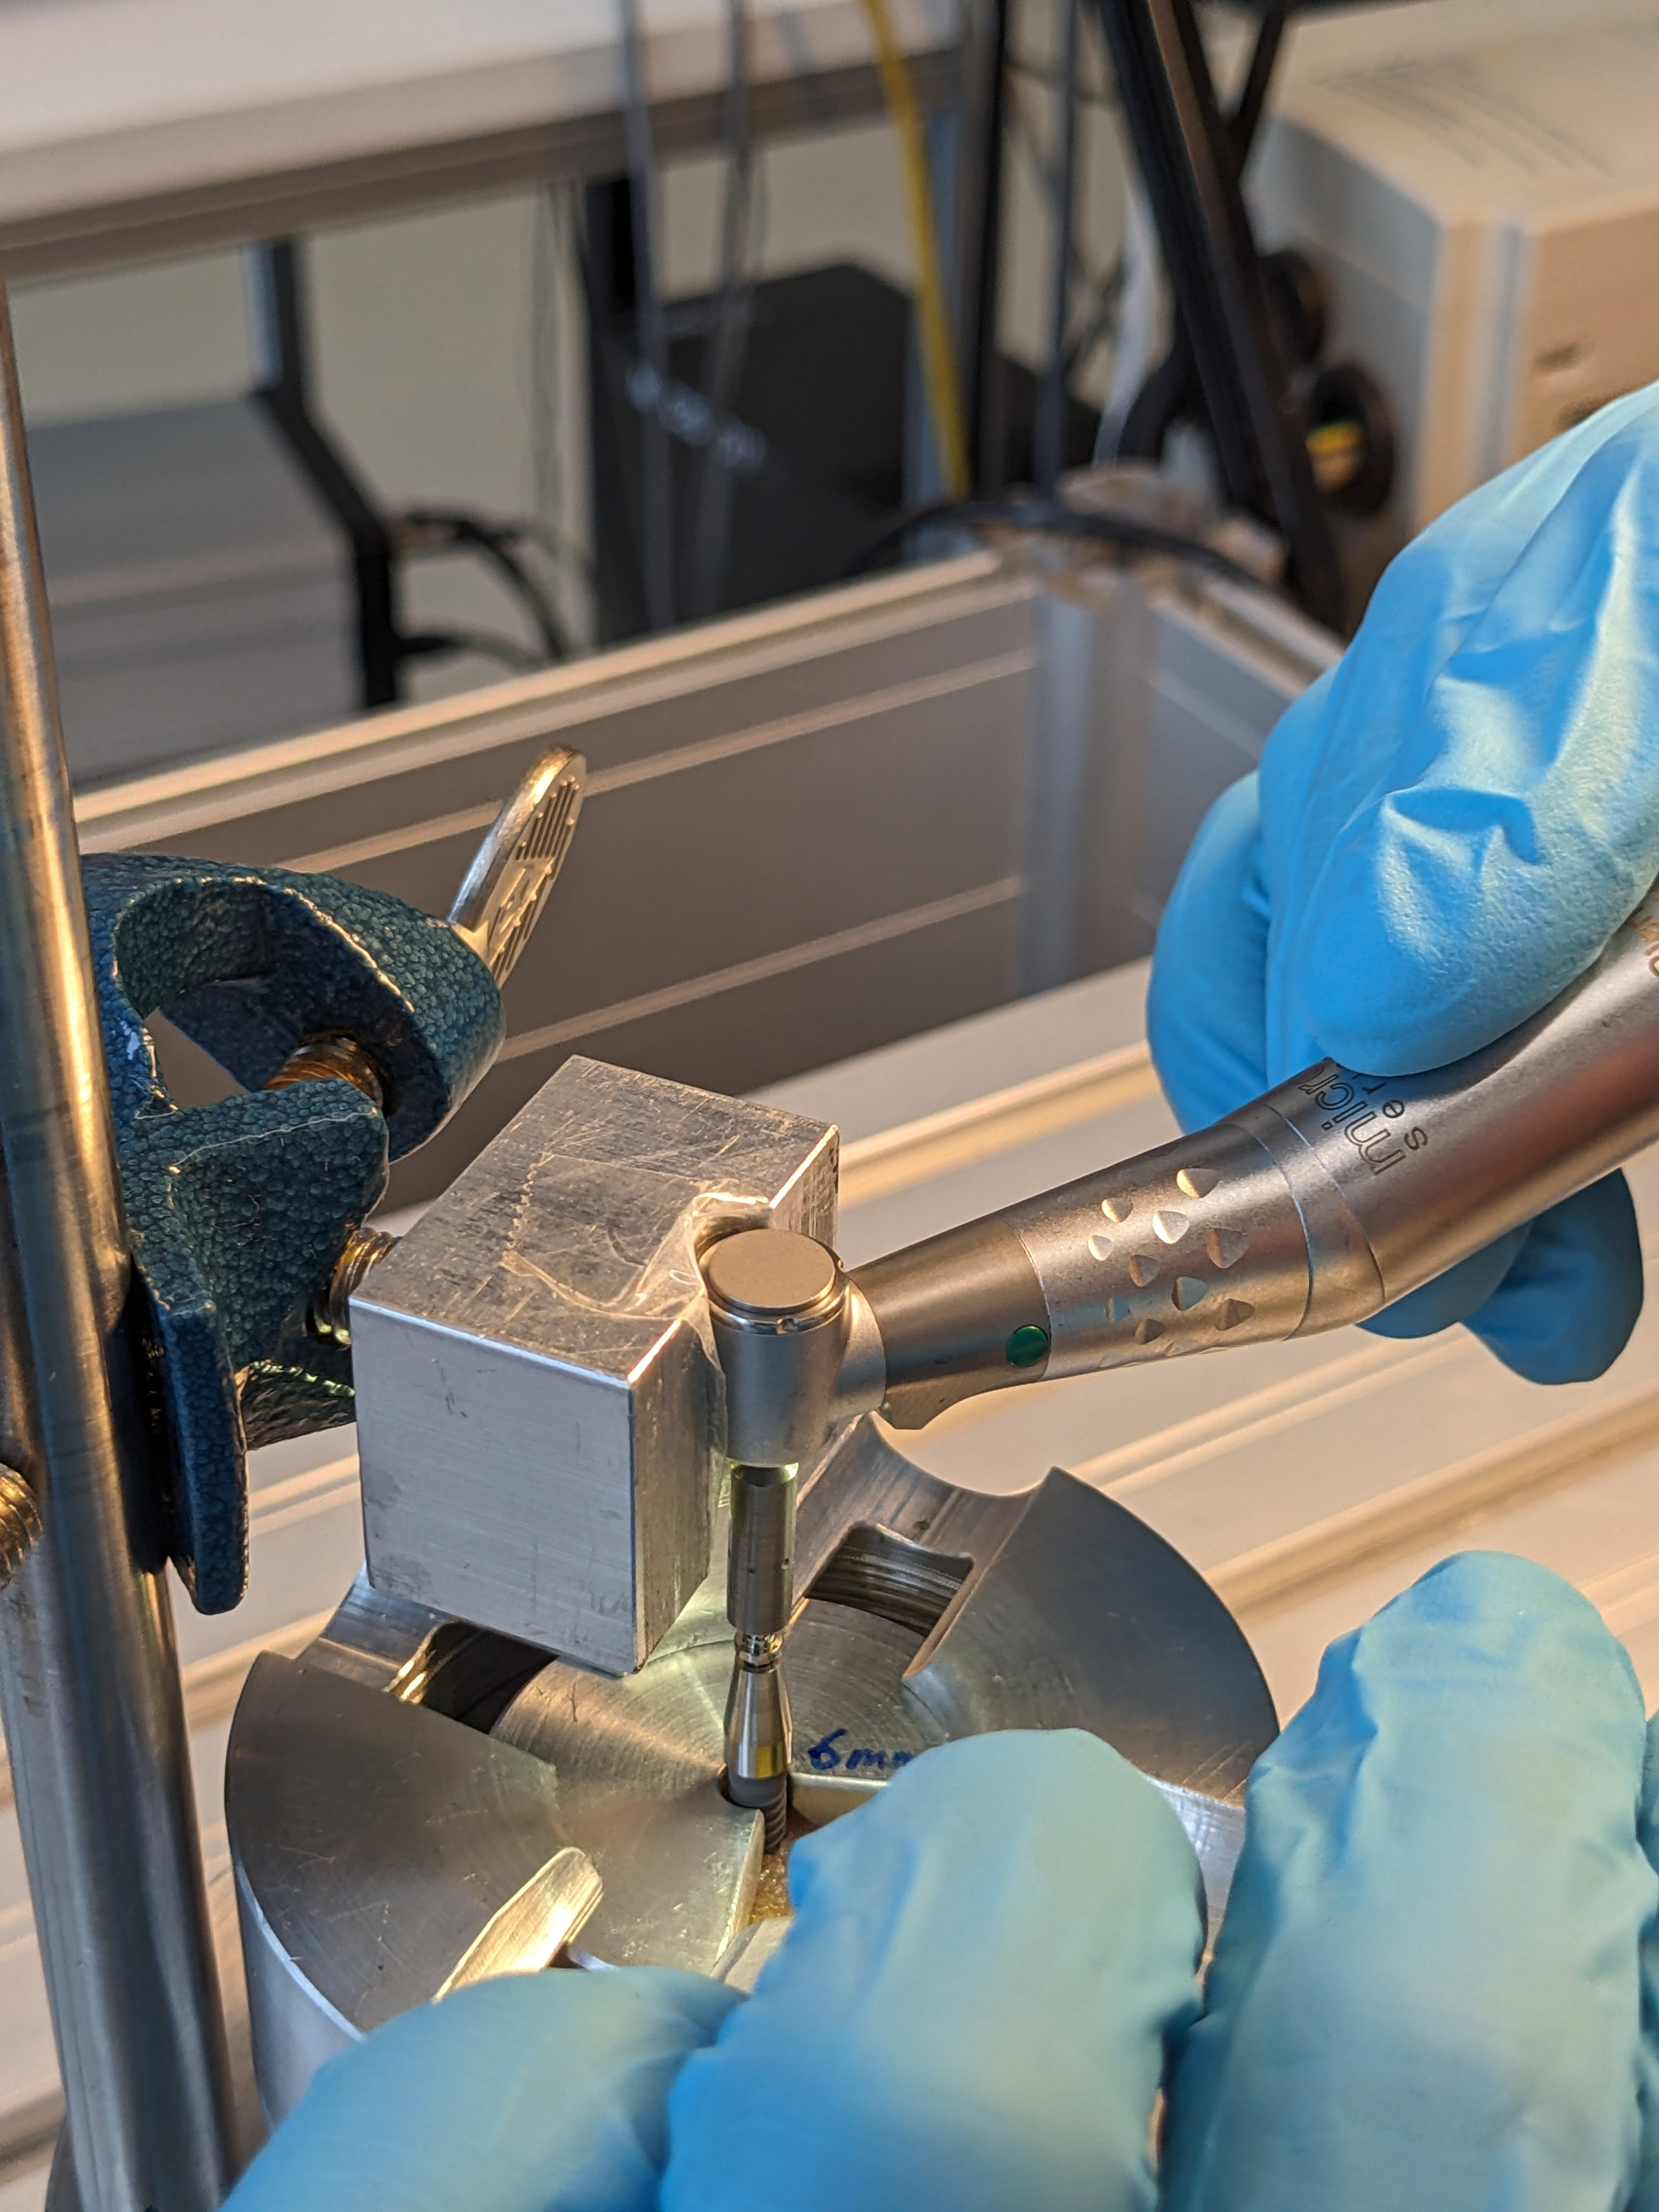
\includegraphics[width=0.4\textwidth]{figures/Experiments/set_implant}}
\subfigure[]{\label{sublable2}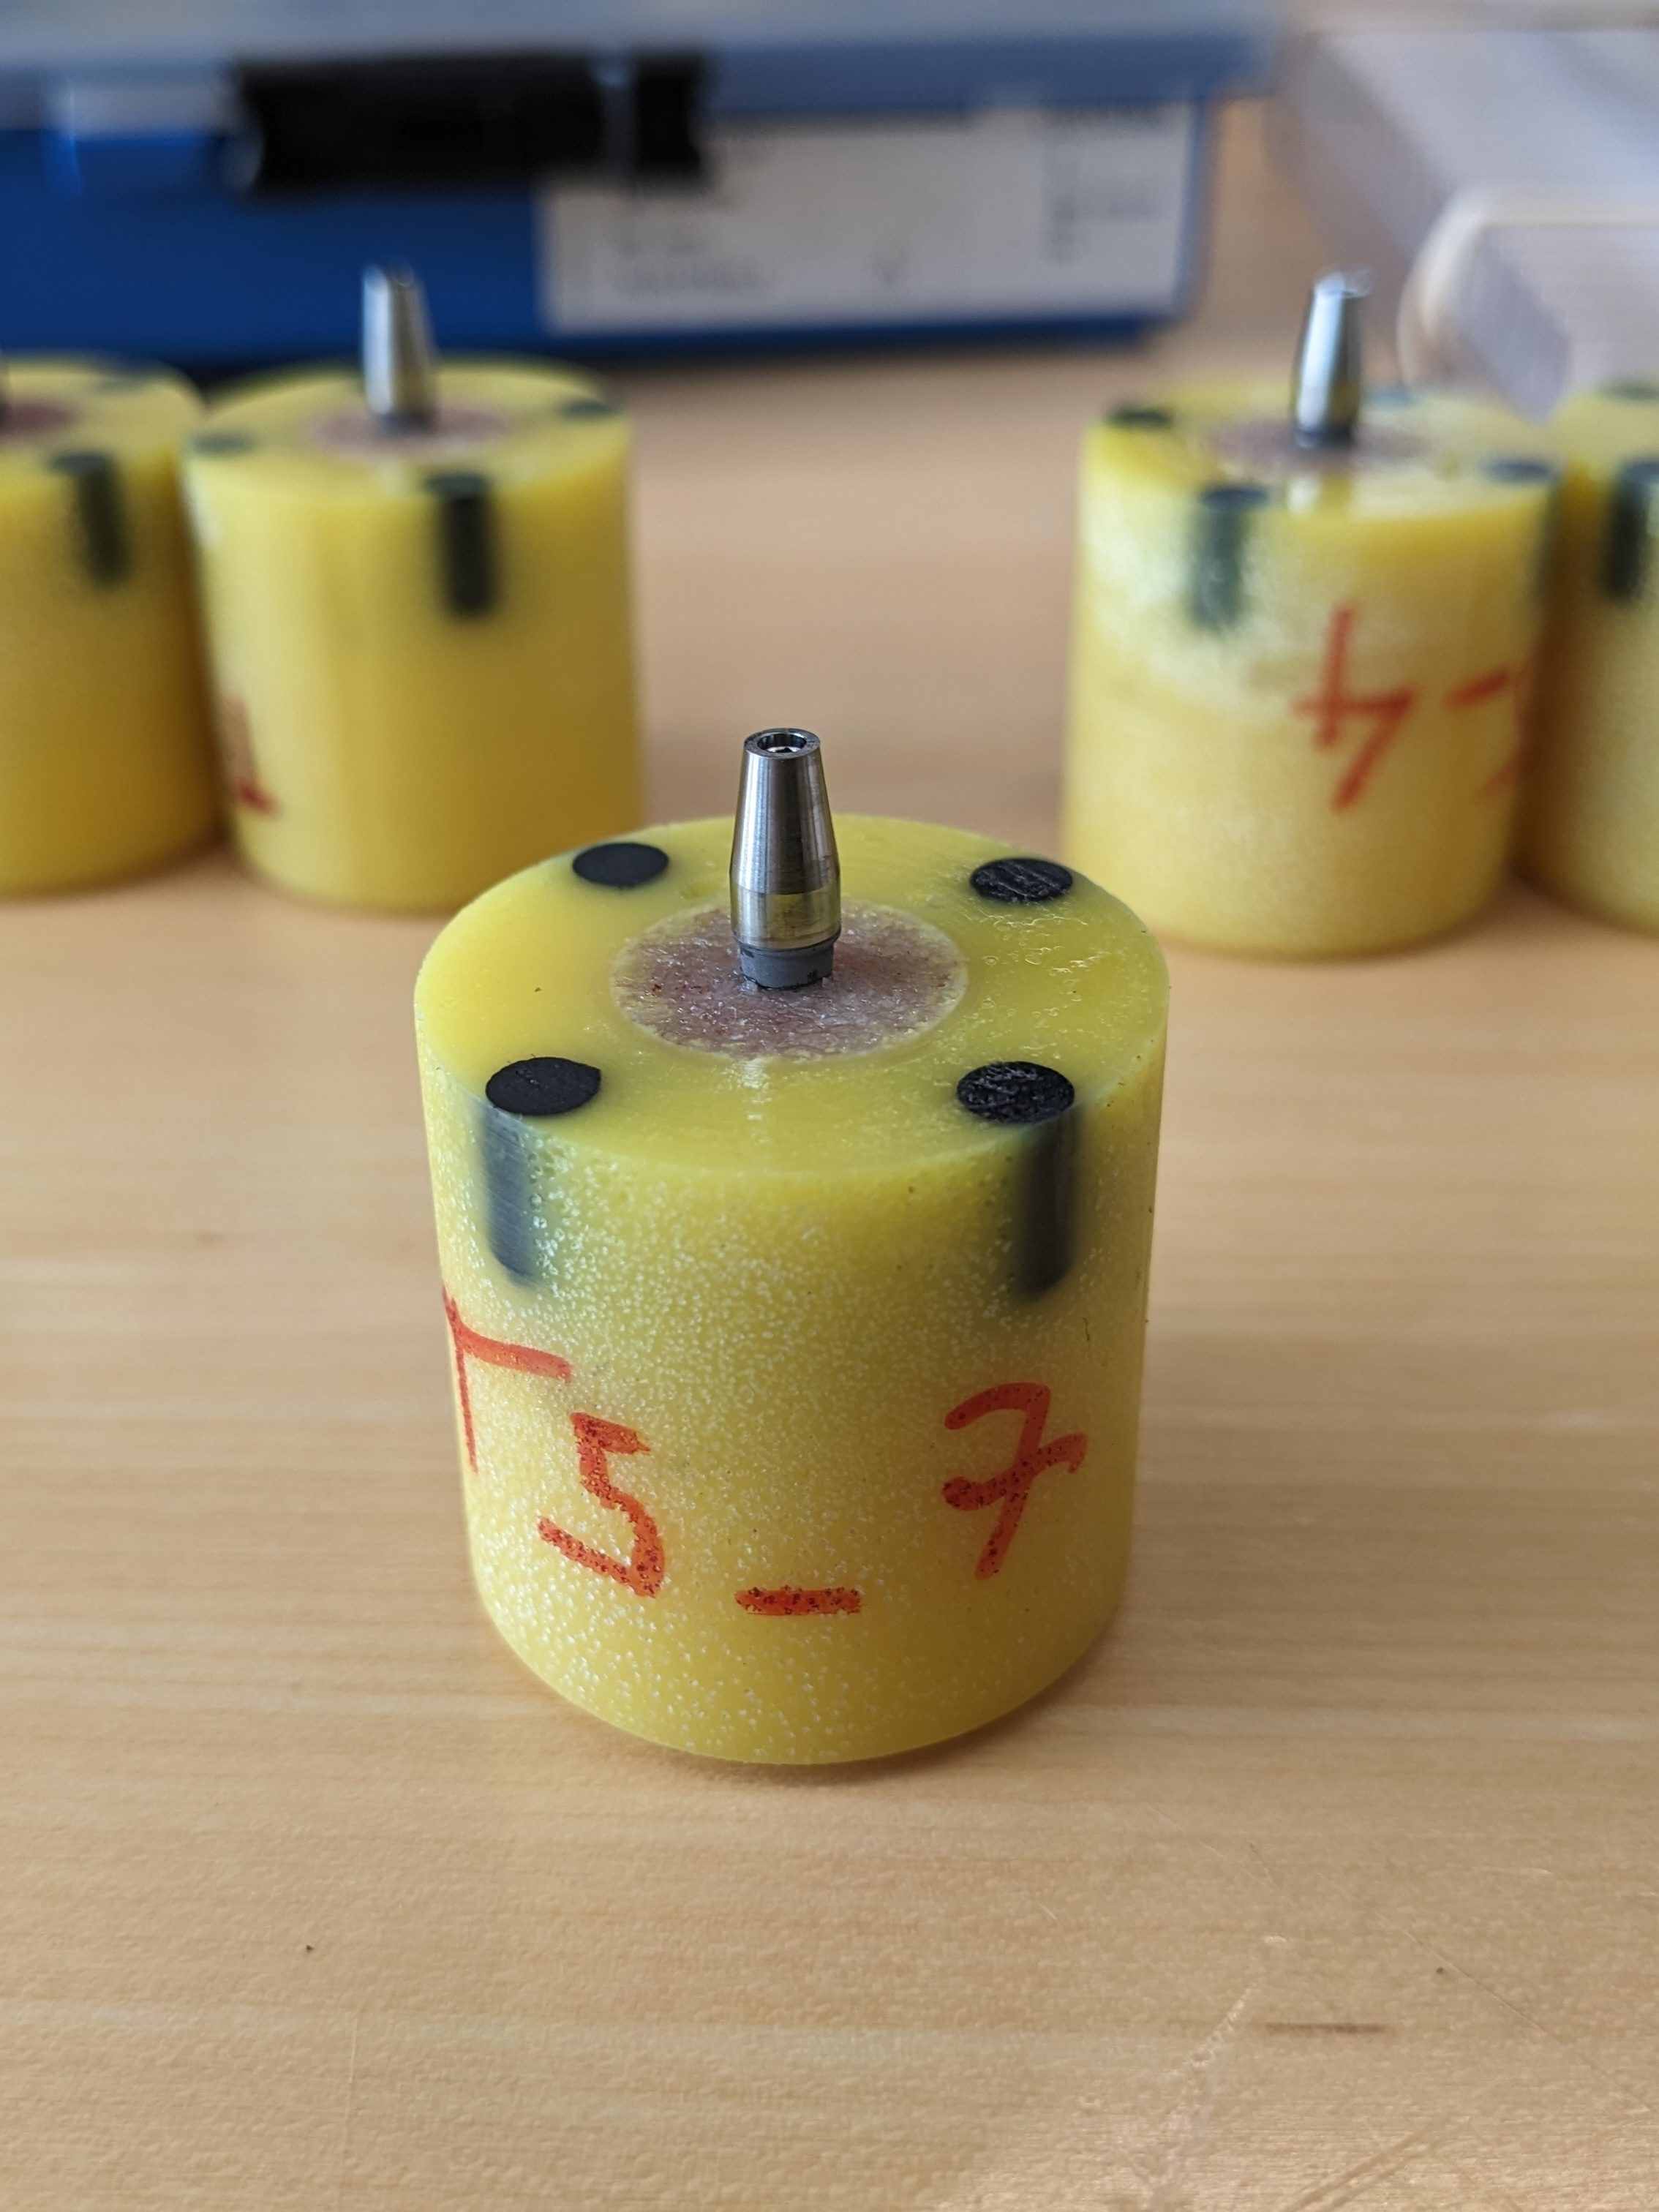
\includegraphics[width=0.4\textwidth]{figures/Experiments/implant_in_bone}}
\captionof{figure}{(a): Implantation setup. (b): Implant in the bovine sample.}
\label{fig:setup}
\end{figure}
%
\subsection{Mechanical Testing}
%
The mechanical testing procedure was carried out in the same way as described by~\citet{thierrin_primary_2022}, which adopted the loading setup from ISO-14801.
The implant was loaded after being tilted 30° along its longitudinal axis.
See fig~\ref{fig:mechanical_setup} for a schematic illustration of the setup.
Following the protocol described in \cite{voumard_intra-operative_2015}, each specimen underwent a displacement-controlled cyclic test with a doubling of displacement up to 2.56~mm to ensure that a failure could be detected within the measurement.
Finally, the maximum stiffness (during the second increment at approximately 50 N) and the ultimate force (UF) were calculated as in~\cite{wili_experimental_2021}.
% TODO: do we need an explanation of how we calculated stiffnes and UF?

\begin{figure}[H]
  \centering
      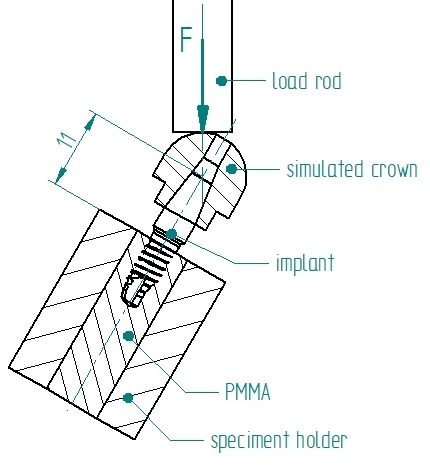
\includegraphics[width=0.5\textwidth]{figures/experiments/mechanical_setup}
  \caption{Drawing of the set-up for the mechanical test with its components.}
  \label{fig:mechanical_setup}
\end{figure} 

As the aim of the study was to compare the two implant systems, no compliance test was performed.
The stiffness values can therefore only be used for comparison between groups and not as absolute values.

\section{Statistical Analysis}
To evaluate the hypotheses, each group was examined for insertion torque, stiffness and ultimate force.
All evaluations were made on the log-log scale to improve the residual distributions.
First, a simple linear regression was plotted with BV/TV as the independent variable and each of the variables of interest as explanatory variables.
In addition to the linear regression, an ANCOVA (controlled for BV/TV) was performed to determine the effect of the different implant types on the values of interest.
Post hoc analysis was performed with a Bonferroni adjustment to test for statistical differences between the two groups by evaluating the estimated marginal means.

\chapter{Results}
%
\section{Experiments}
The results of the statistical analysis described above are presented in this section.

\newpage
%
%
% TODO: for all following sections: 
% - make log-log plot.
% - make axis normal numbers, not log-nubmer
% - make ANCOVA in log-log
% - make Box-Plot _not_ in log-log
\subsection{Insertion torque}
%
\begin{figure}[H]
\centering 
\subfigure[]{\label{sublable2}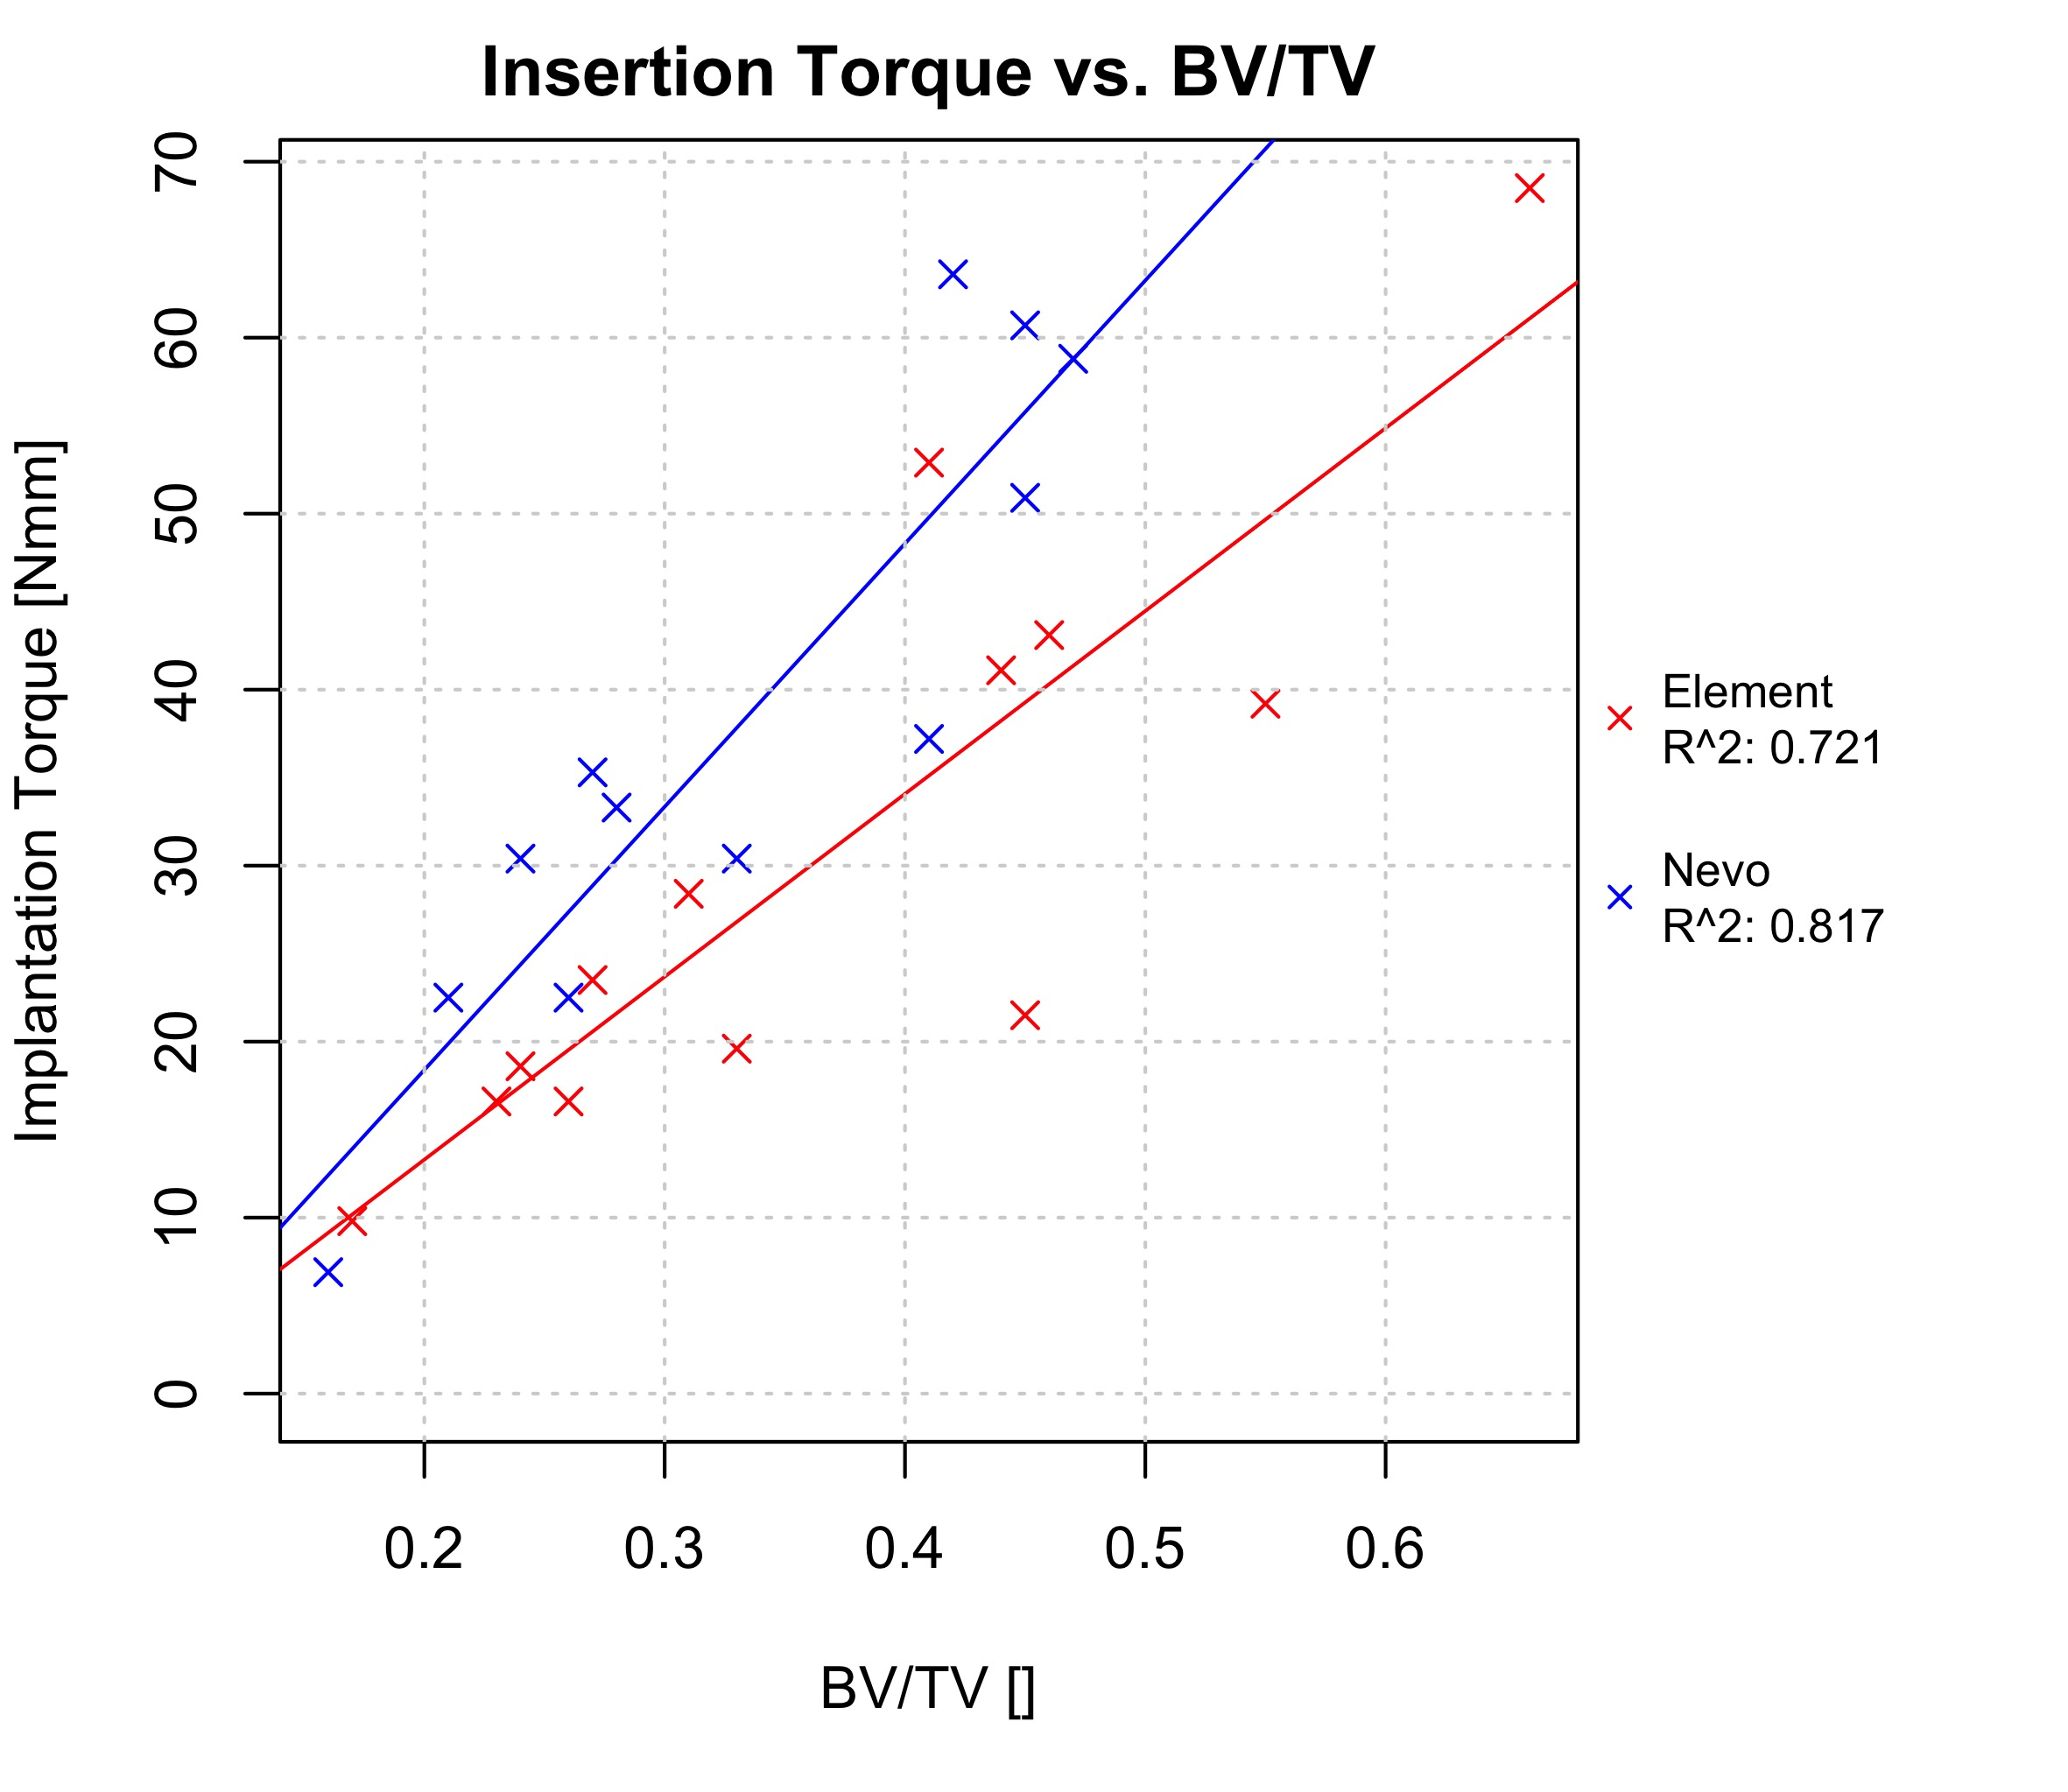
\includegraphics[width=0.49\textwidth]{figures/EXP_IT}}
\subfigure[]{\label{sublable2}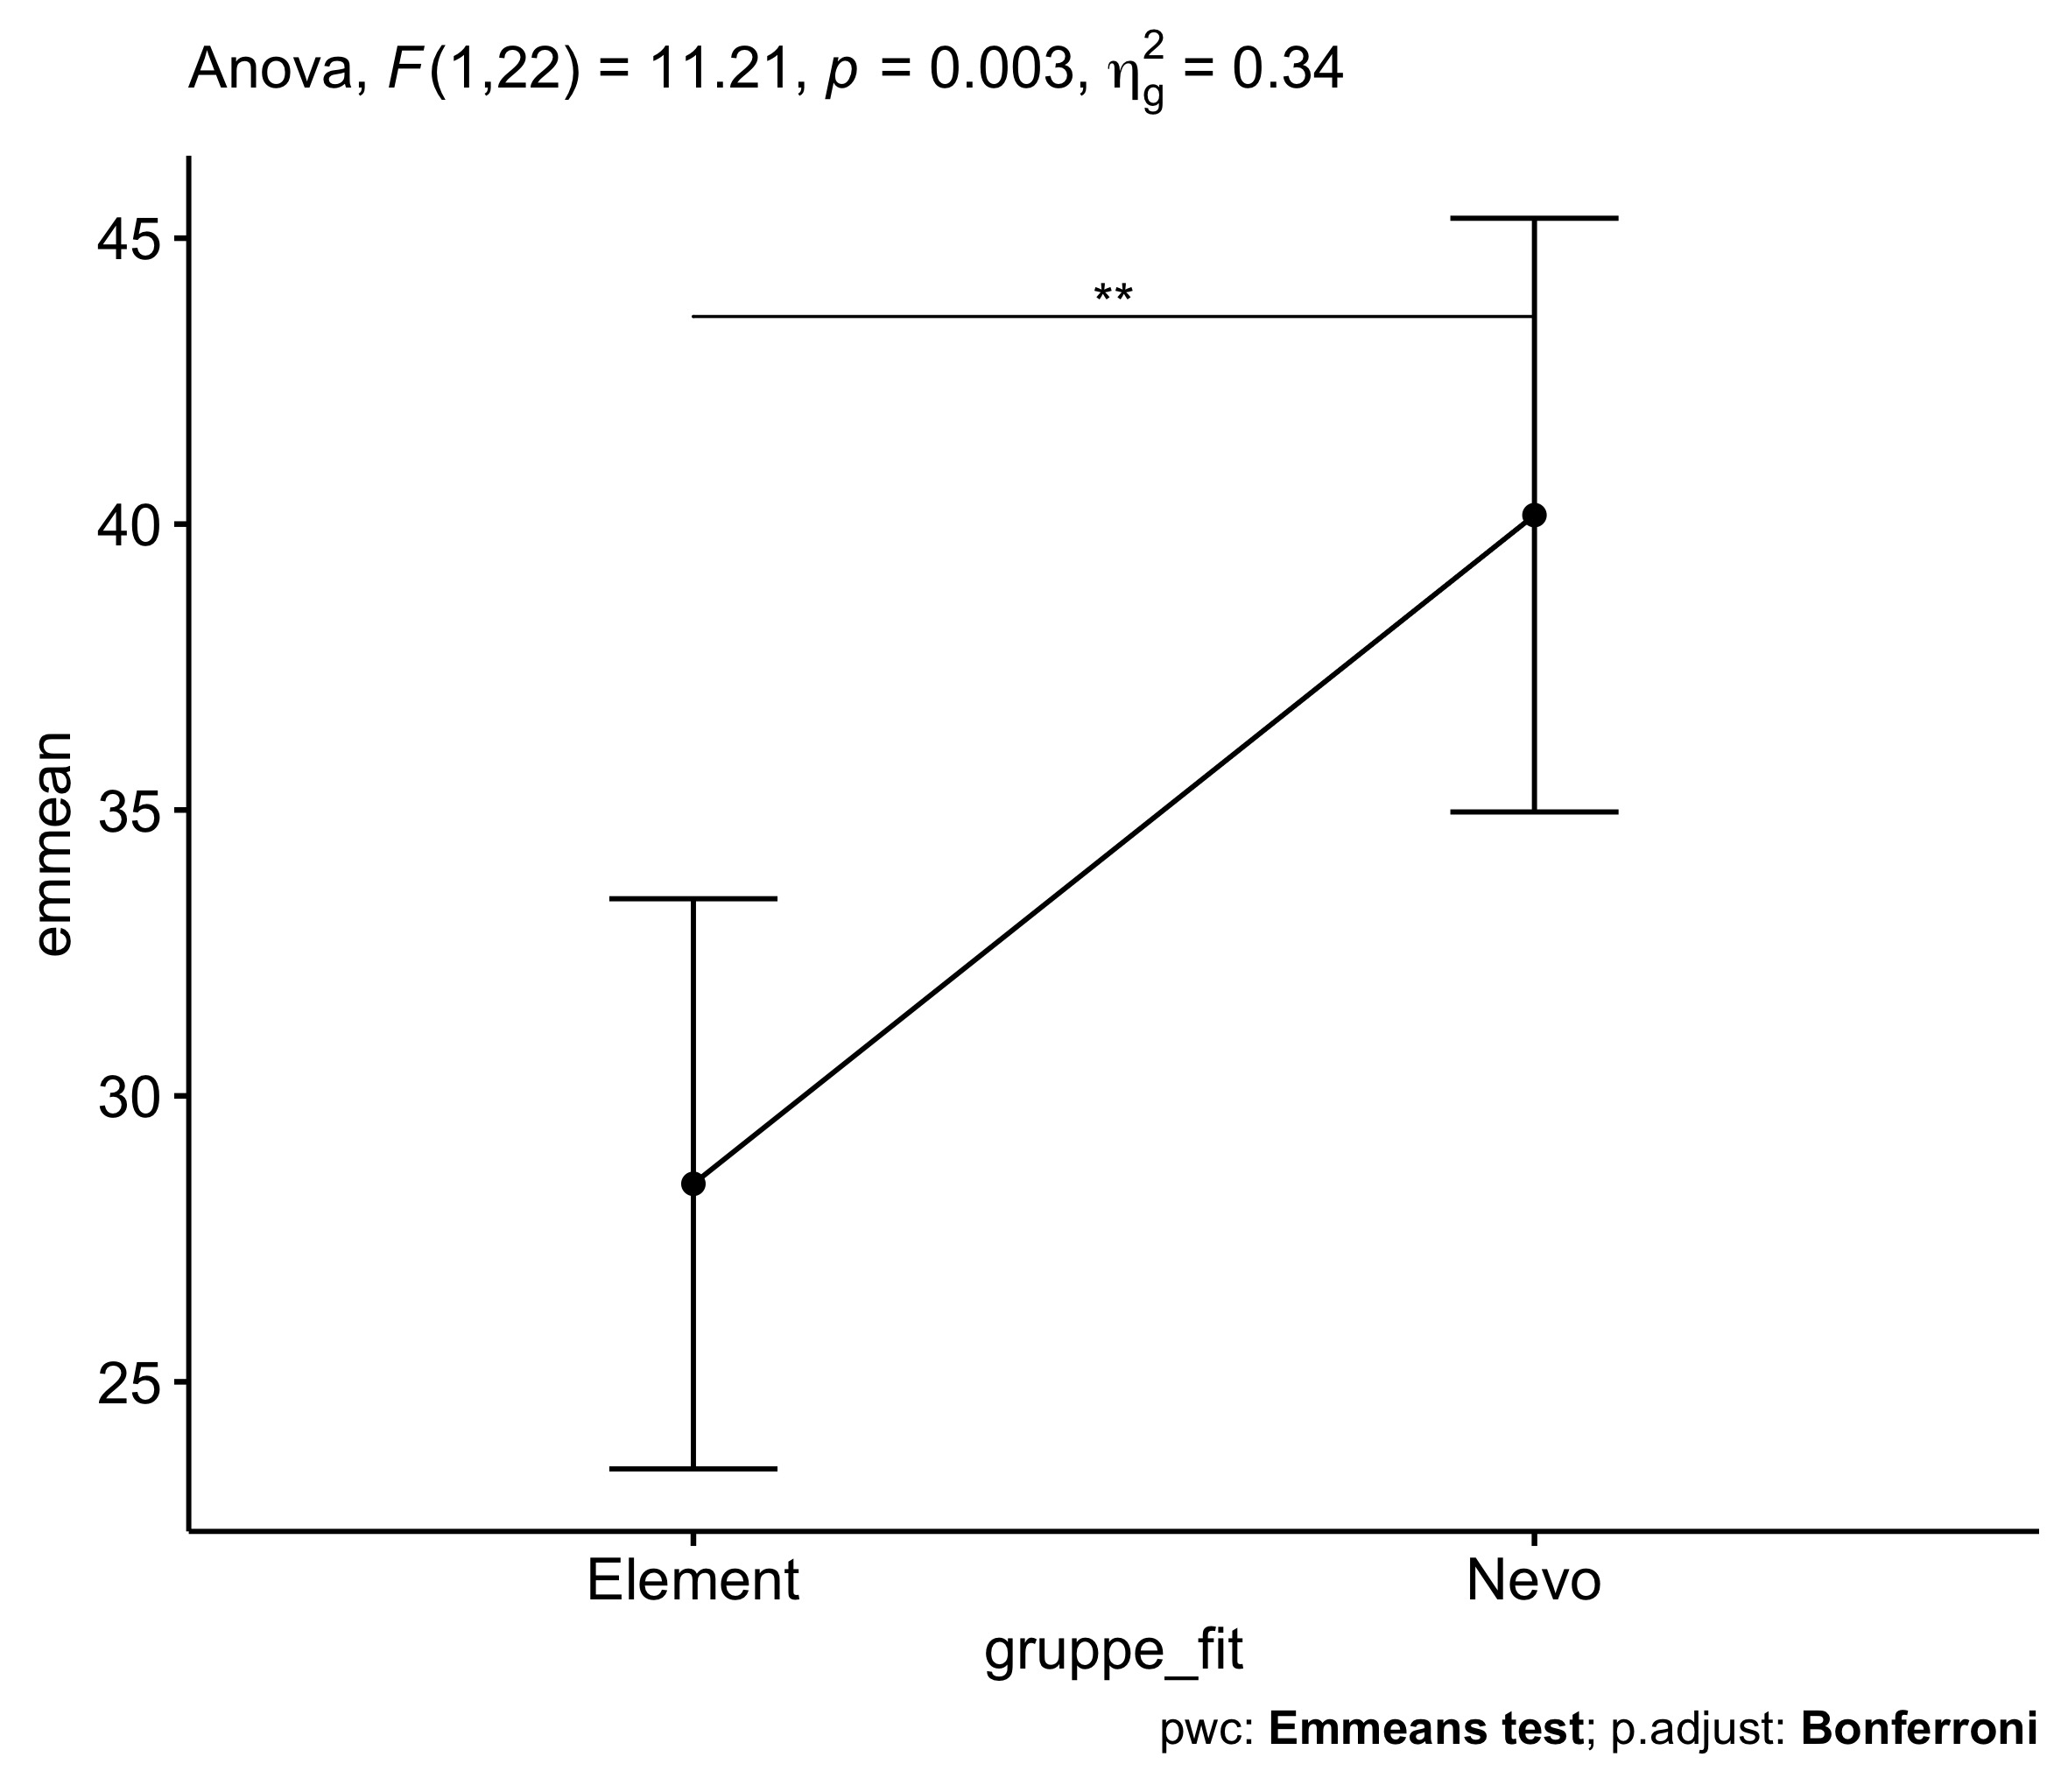
\includegraphics[width=0.49\textwidth]{figures/emmenas_IT}}
\captionof{figure}{(a): Insertion torque as a function of BV/TV with the individual linear regression model of each group. (b): Box plot of the estimated marginal means (emmeans or least square means) of each group after Bonferroni correction, controlled with BV/TV as covariate.}
\label{fig:RM_exp}
\end{figure}
%
\begin{table}[H]
\centering
\resizebox{300pt}{!}{%
\begin{tabular}{|l|c|c|c|c||c|}
	\hline
	& \multicolumn{4}{c||}{individual lin. regression} & eval. ANCOVA (log)\\
	\hline 
	Group & $R^2$ & p-value & mean & CV & emmean $\pm$ 95\%conf.\\
	\hline
	ELEMENT & 0.76 & 5.18e-5 & 30.72 & 0.56 & 3.22 $\pm$ 0.15\\
	\hline
	NEVO & 0.80 & 5.35e-5 & 37.71 & 0.46 & 3.56 $\pm$ 0.16\\
	\hline
\end{tabular}
}
\caption{Results for the linear regression (RSE: residual standard error, CV: coefficient of variation) of the experimentally evaluated implanting torque values. And the evaluation of the ANCOVA by the emmenas after Bonferroni correction.}
\label{tab:it_results}
\end{table}
%
\begin{table}[H]
\centering
\resizebox{200pt}{!}{%
\begin{tabular}{|l|c|c|c|c|c|c|}
	\hline 
	Effect & DFn & DFd & F & p & ges\\
	\hline
	\hline
	bvtv (log) & 1 & 22 & 83.81 & 5.87e-9 & 0.445\\
	\hline
	group & 1 & 22 & 9.772 & 5.00e-3 & 0.308\\
	\hline
\end{tabular}
}
\caption{Results from the ANCOVA analysis, controlling for BV/TV.}
\label{tab:it_ancova}
\end{table}
%
% G1 and G2 showed a significant linear relationship between implantation torque (IT) and BV/TV, where IT increases with increasing BV/TV. The linear relation in G3 is not significant but showed a tendency to the same behavior as the others.\\
% \\
An overview of the statistical metrics can be found in the table~\ref{tab:it_results}.
The ANCOVA indicated that the insertion torque was significantly related to the BV$/$TV of the sample, F(1,22)=83.81, p$<$0.001.
In addition, after controlling for the effect of BV$/$TV, there was a significant difference between the groups on insertion torque with F(1,22)$=$9.772 and p$<$0.05.
See table~\ref{tab:it_ancova} for details.

In a further analysis, the homogeneity of the regression slopes was analysed with an interaction term.
However, it was not statistically significant at p$>$0.05.

% The ANCOVA pointed out that globally (over all groups) the insertion torque was significantly related to the sample's BV$/$TV, F(1,24)$=$41.5, p$<$0.001. Further more, there was a significant difference between the groups on the insertion torque after controlling for the effect of the BV$/$TV, F(2,24)$=$45.7, p$<$0.001.\\
% Through the post hoc analysis it could be observed that the emmeans of the insertion torque was significantly greater in G2 (169.0 Nmm) compared to G1 (110.0 Nmm) and G3 (52.3 Nmm) and G1 was greater than G3, p$<$0.001.
%
%
%
\subsection{Stiffness}
%
\begin{figure}[H]
\centering 
\subfigure[]{\label{sublable2}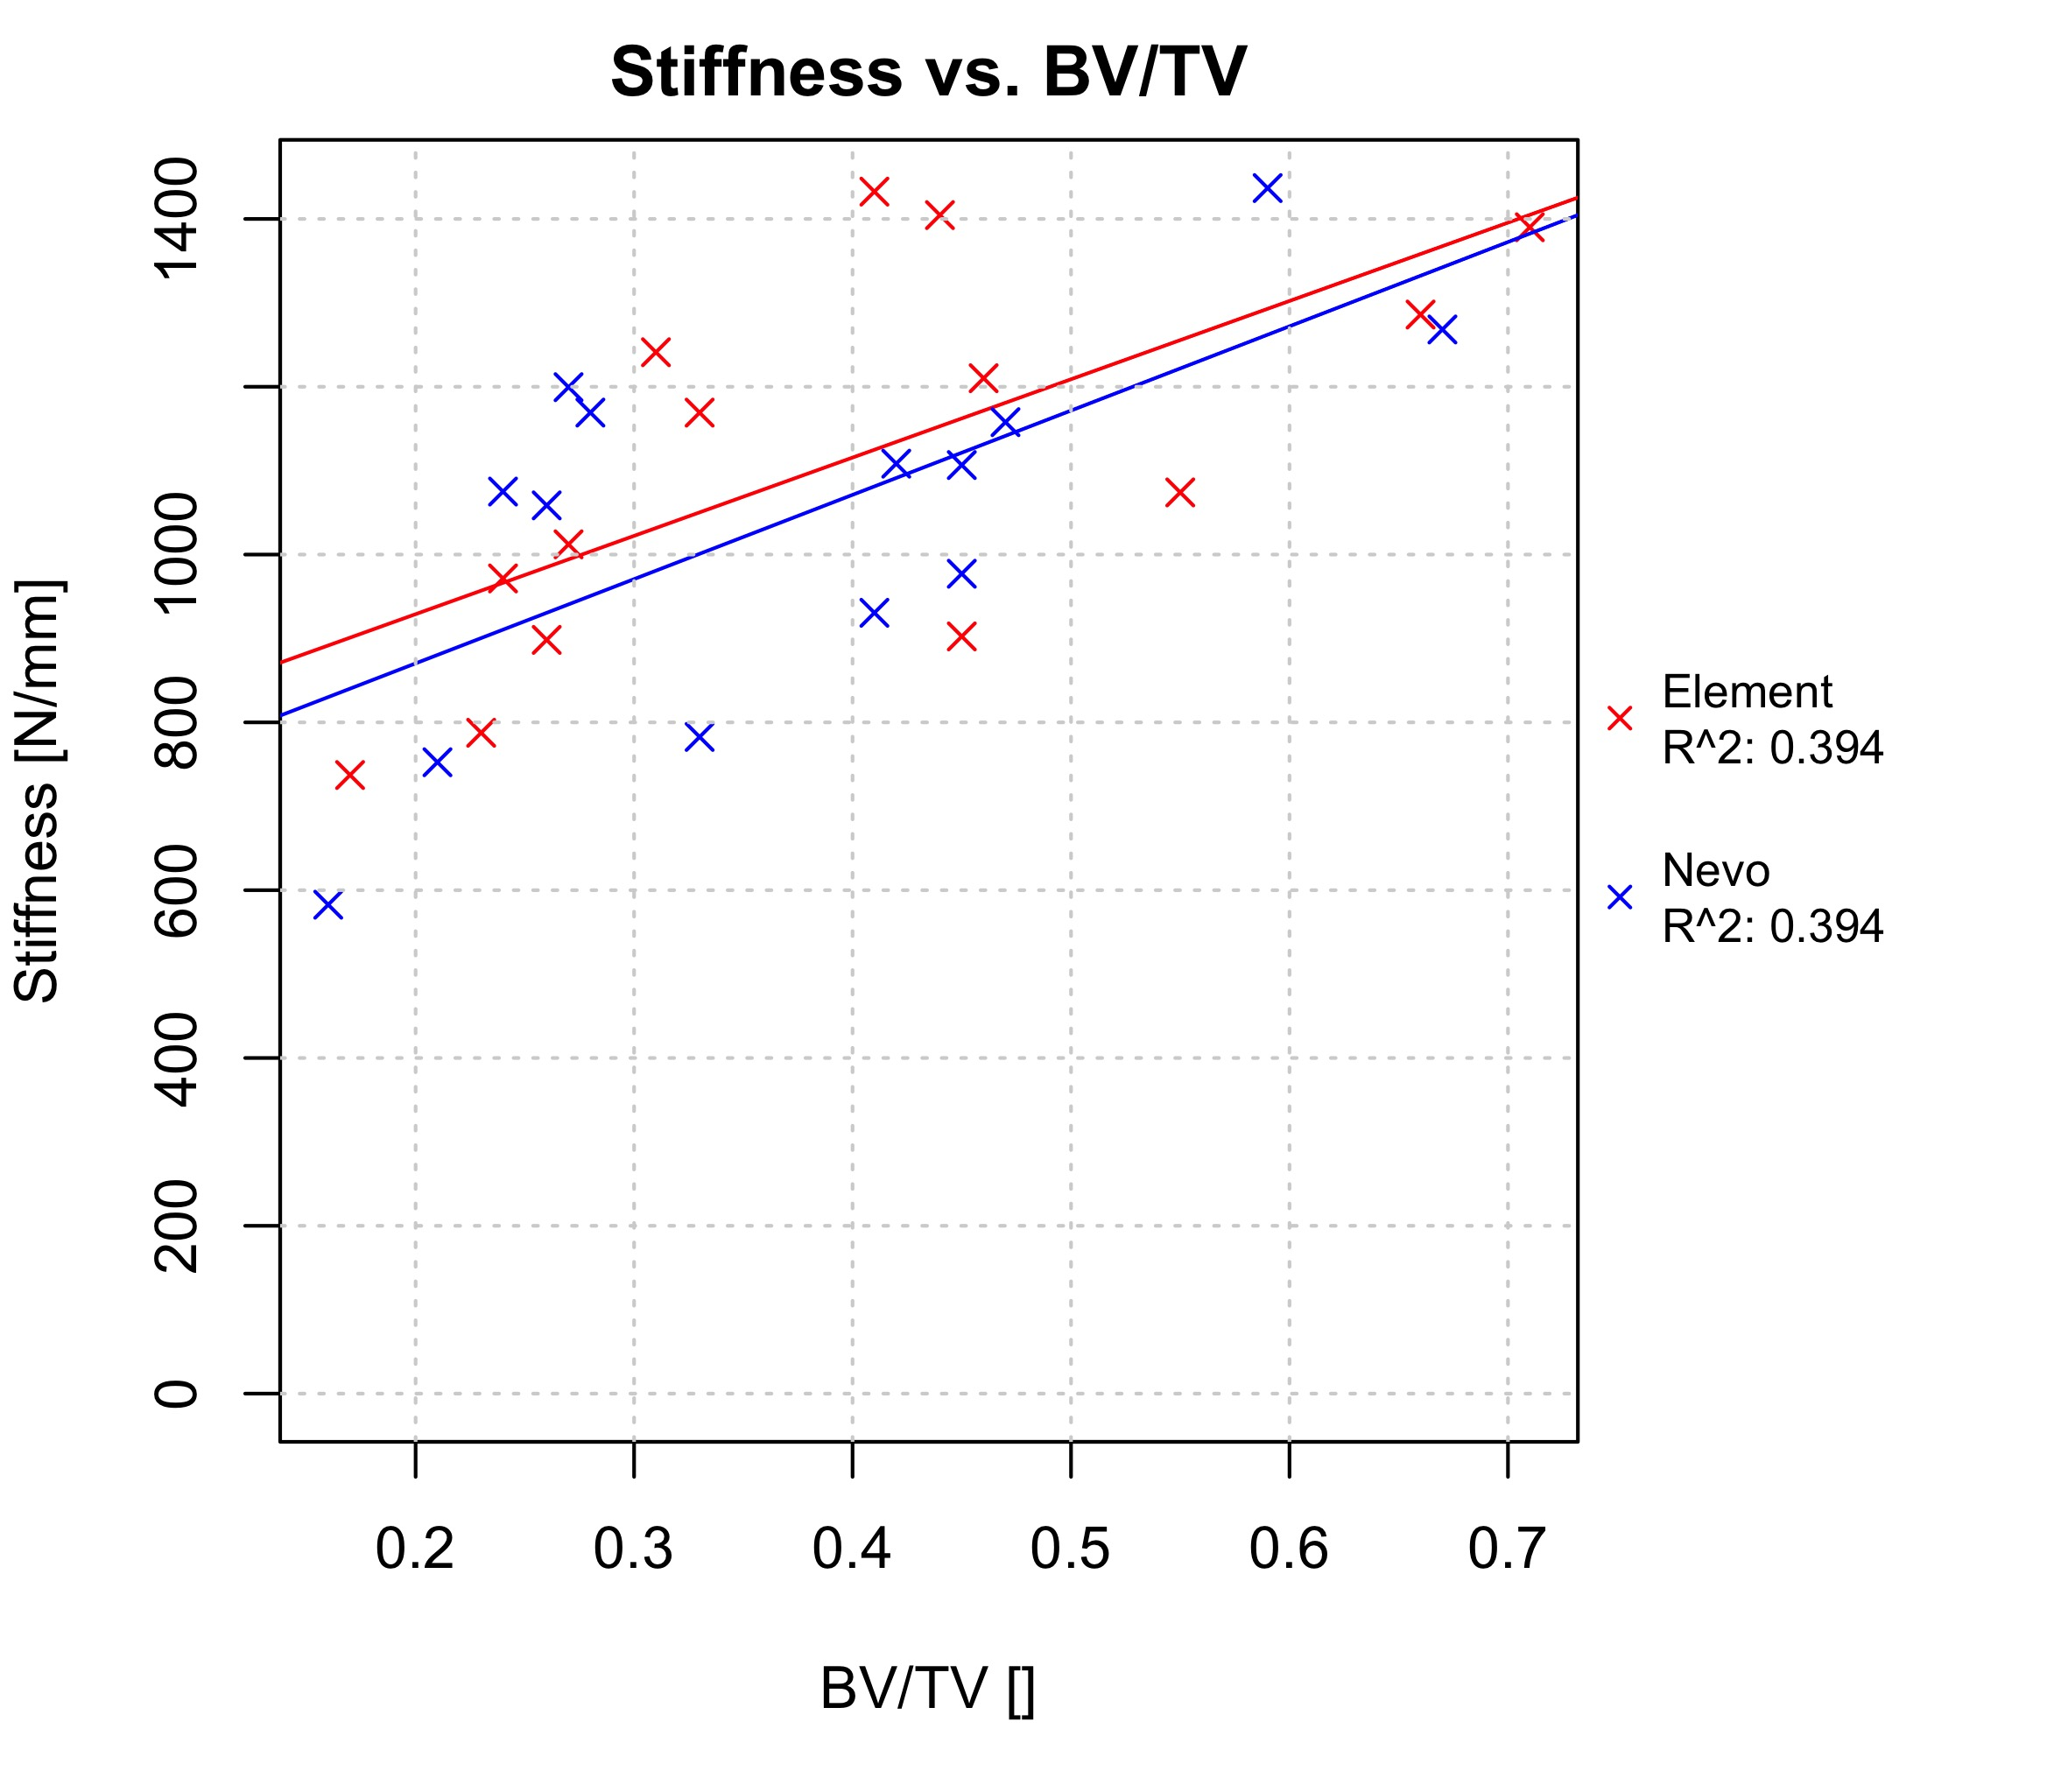
\includegraphics[width=0.49\textwidth]{figures/EXP_ST}}
\subfigure[]{\label{sublable2}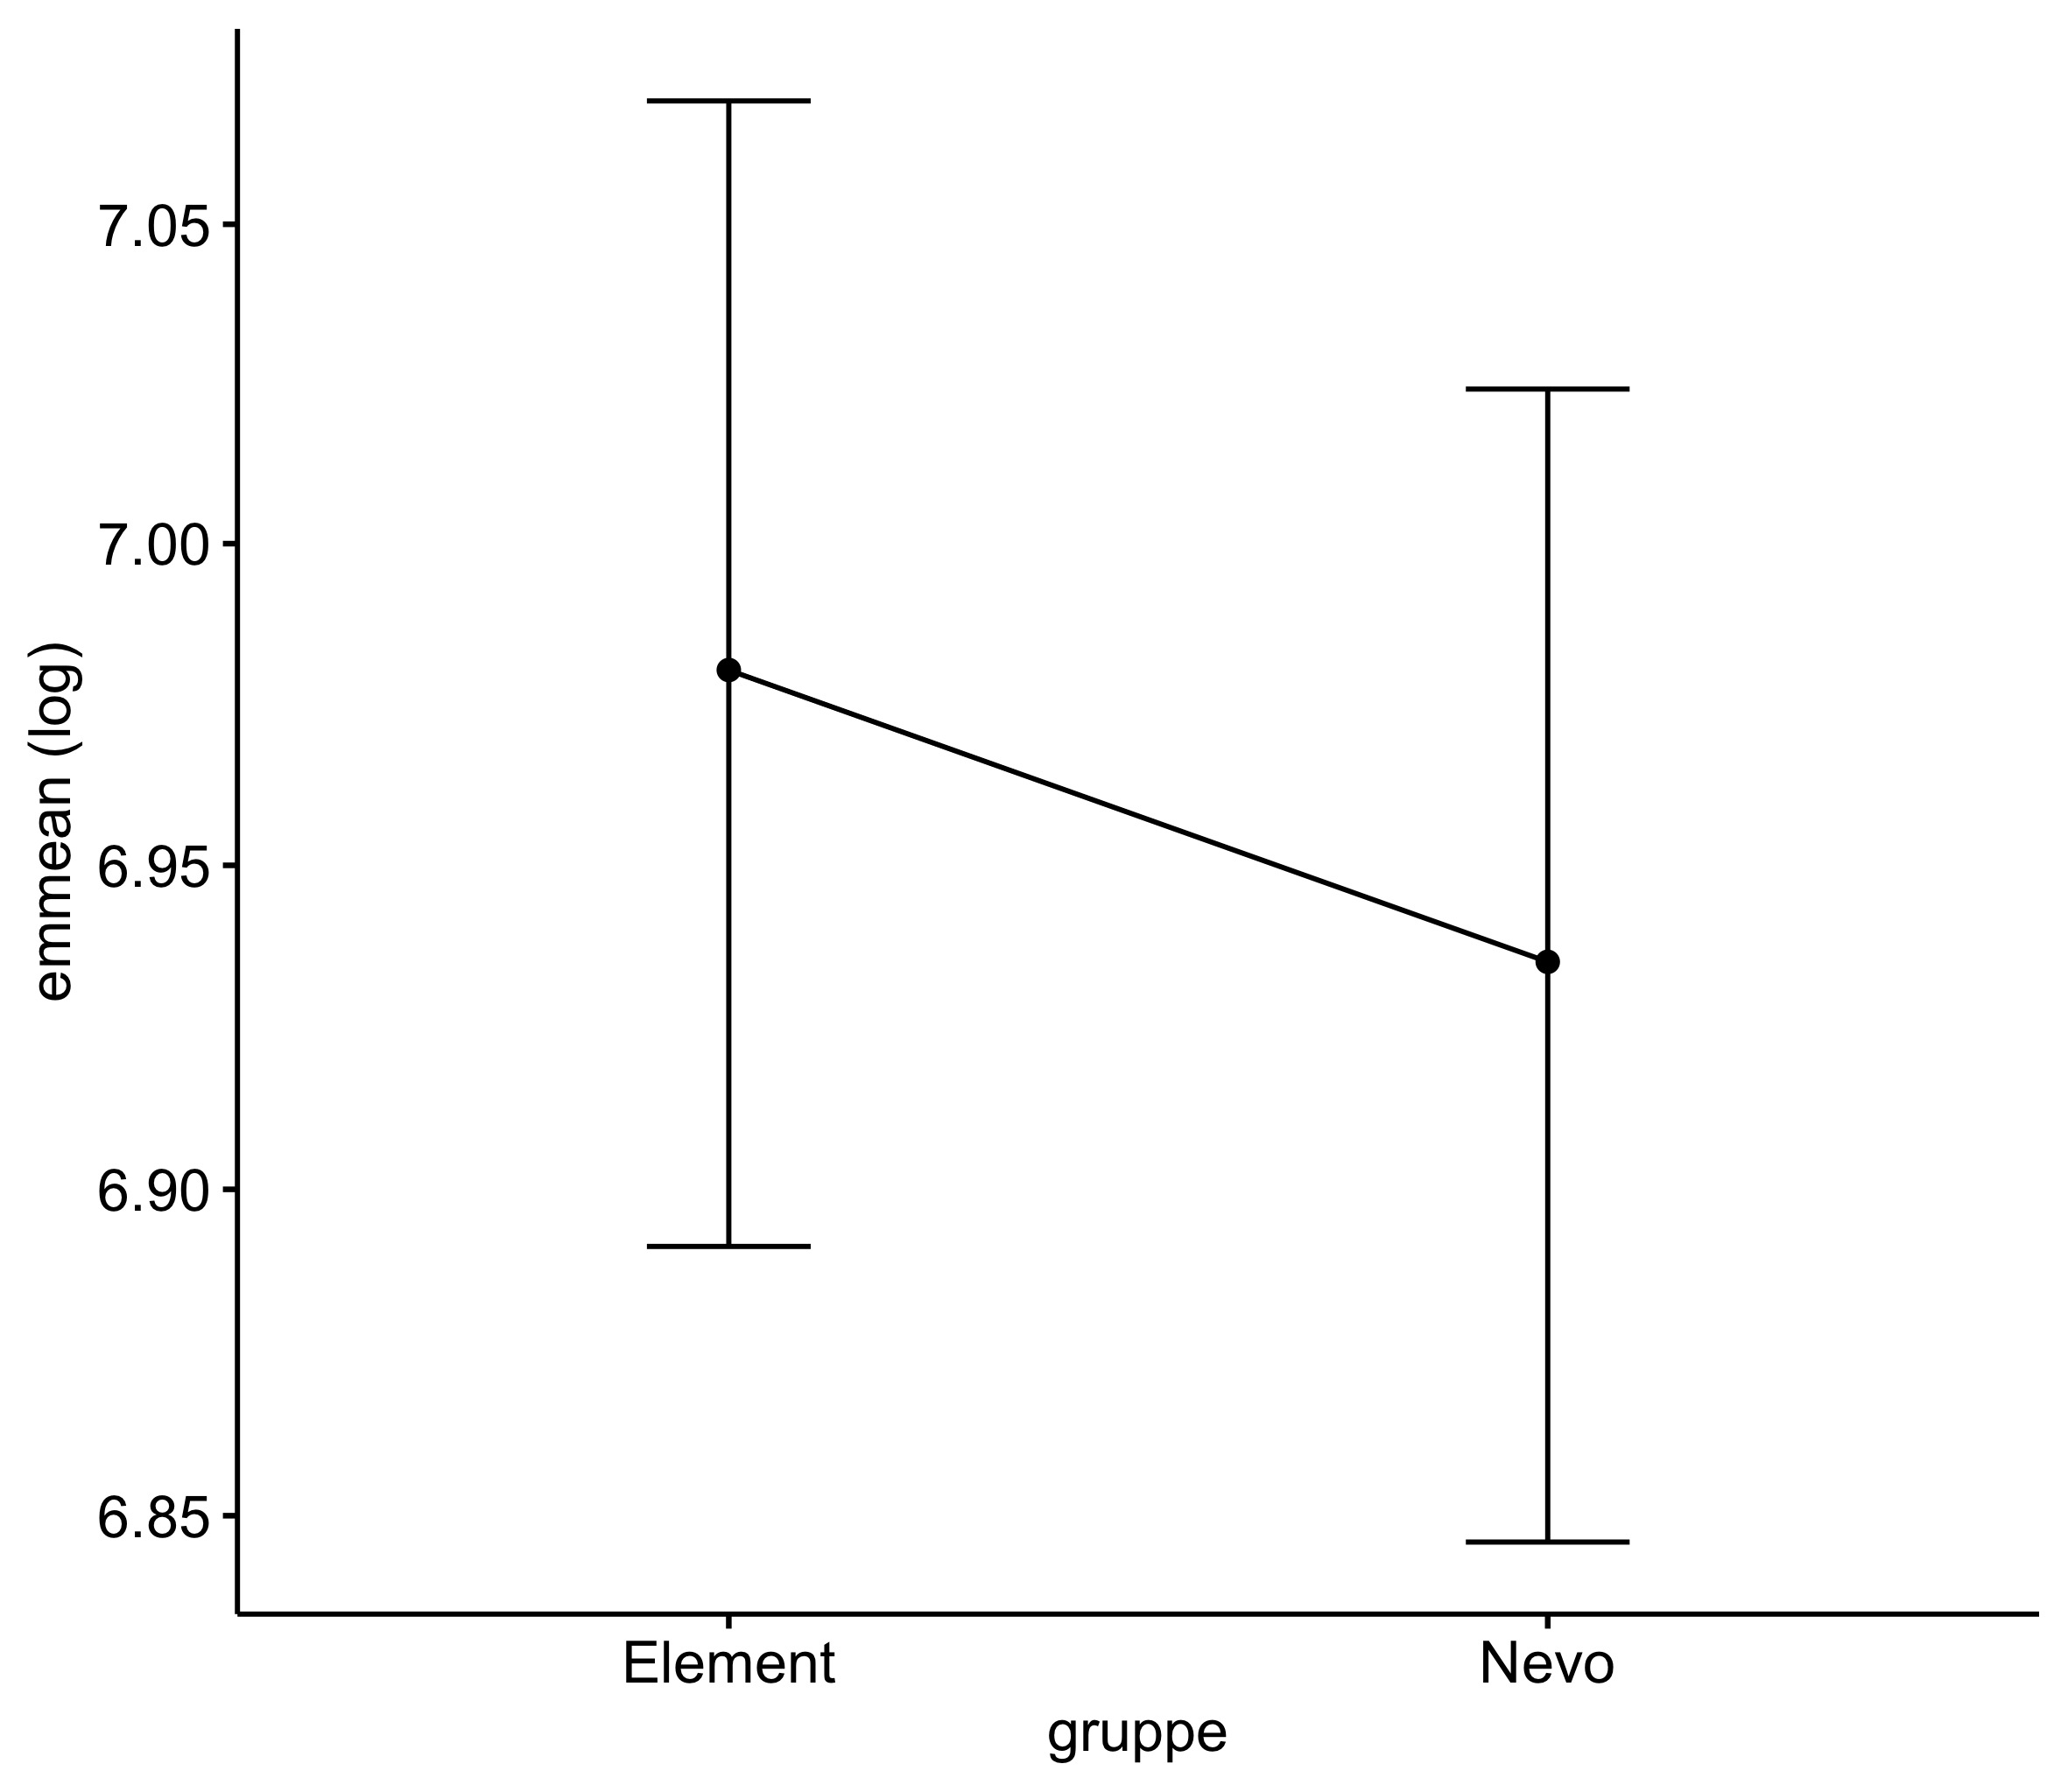
\includegraphics[width=0.49\textwidth]{figures/emmenas_ST}}
\captionof{figure}{(a): Insertion torque as a function of BV/TV with the individual linear regression model of each group. (b): Box plot of the estimated marginal means (emmeans or least square means) of each group after Bonferroni correction, controlled with BV/TV as covariate.}
\label{fig:RM_exp}
\end{figure}
%
\begin{table}[H]
\centering
\resizebox{300pt}{!}{%
\begin{tabular}{|l|c|c|c|c||c|}
	\hline
	& \multicolumn{4}{c||}{individual lin. regression} & eval. ANCOVA (log)\\
	\hline 
	Group & $R^2$ & p-value & mean & CV & emmean $\pm$ 95\%conf.\\
	\hline
	ELEMENT & 0.50 & 2.74 & 1108.36 & 0.21 & 6.98 $\pm$ 0.09\\
	\hline
	NEVO & 0.43 & 6.18e-3 & 1043.27 & 0.21 & 6.94 $\pm$ 0.09\\
	\hline
\end{tabular}
}
	\caption{Results for the linear regression (RSE: residual standard error, CV: coefficient of variation) of the experimentally evaluated stiffness values. And the evaluation of the ANCOVA by the emmenas after Bonferroni correction and controlling for BV/TV.}
\label{tab:st_results}
\end{table}
%
\begin{table}[H]
\centering
\resizebox{200pt}{!}{%
\begin{tabular}{|l|c|c|c|c|c|c|}
	\hline 
	Effect & DFn & DFd & F & p & ges\\
	\hline
	\hline
	bvtv (log) & 1 & 25 & 26.174 & 2.76e-9 & 0.511\\
	\hline
	group & 1 & 25 & 0.546 & 4.67e-1 & 0.021\\
	\hline
\end{tabular}
}
\caption{Results from the ANCOVA analysis, controlling for BV/TV.}
\label{tab:st_ancova}
\end{table}
%
% G1 and G2 showed a significant linear relationship between implantation torque (IT) and BV/TV, where IT increases with increasing BV/TV. The linear relation in G3 is not significant but showed a tendency to the same behavior as the others.\\
% \\
An overview of the statistical metrics can be found in the table~\ref{tab:st_results}.
The ANCOVA indicated that stiffness was significantly related to the BV$/$TV of the sample, F(1,22)=26.174, p$<$0.001.
However, after controlling for the effect of BV$/$TV, there was no significant difference between groups in ultimate strength, F(1,25)$=$0.546, p$>$0.05.
See table~\ref{tab:st_ancova} for details.

In a further analysis, the homogeneity of the regression slopes was analysed with an interaction term.
However, it was not statistically significant at p$>$0.05.

% The ANCOVA pointed out that globally (over all groups) the insertion torque was significantly related to the sample's BV$/$TV, F(1,24)$=$41.5, p$<$0.001. Further more, there was a significant difference between the groups on the insertion torque after controlling for the effect of the BV$/$TV, F(2,24)$=$45.7, p$<$0.001.\\
% Through the post hoc analysis it could be observed that the emmeans of the insertion torque was significantly greater in G2 (169.0 Nmm) compared to G1 (110.0 Nmm) and G3 (52.3 Nmm) and G1 was greater than G3, p$<$0.001.
%
%
%
\subsection{Ultimate Force}
%
\begin{figure}[H]
\centering 
\subfigure[]{\label{sublable2}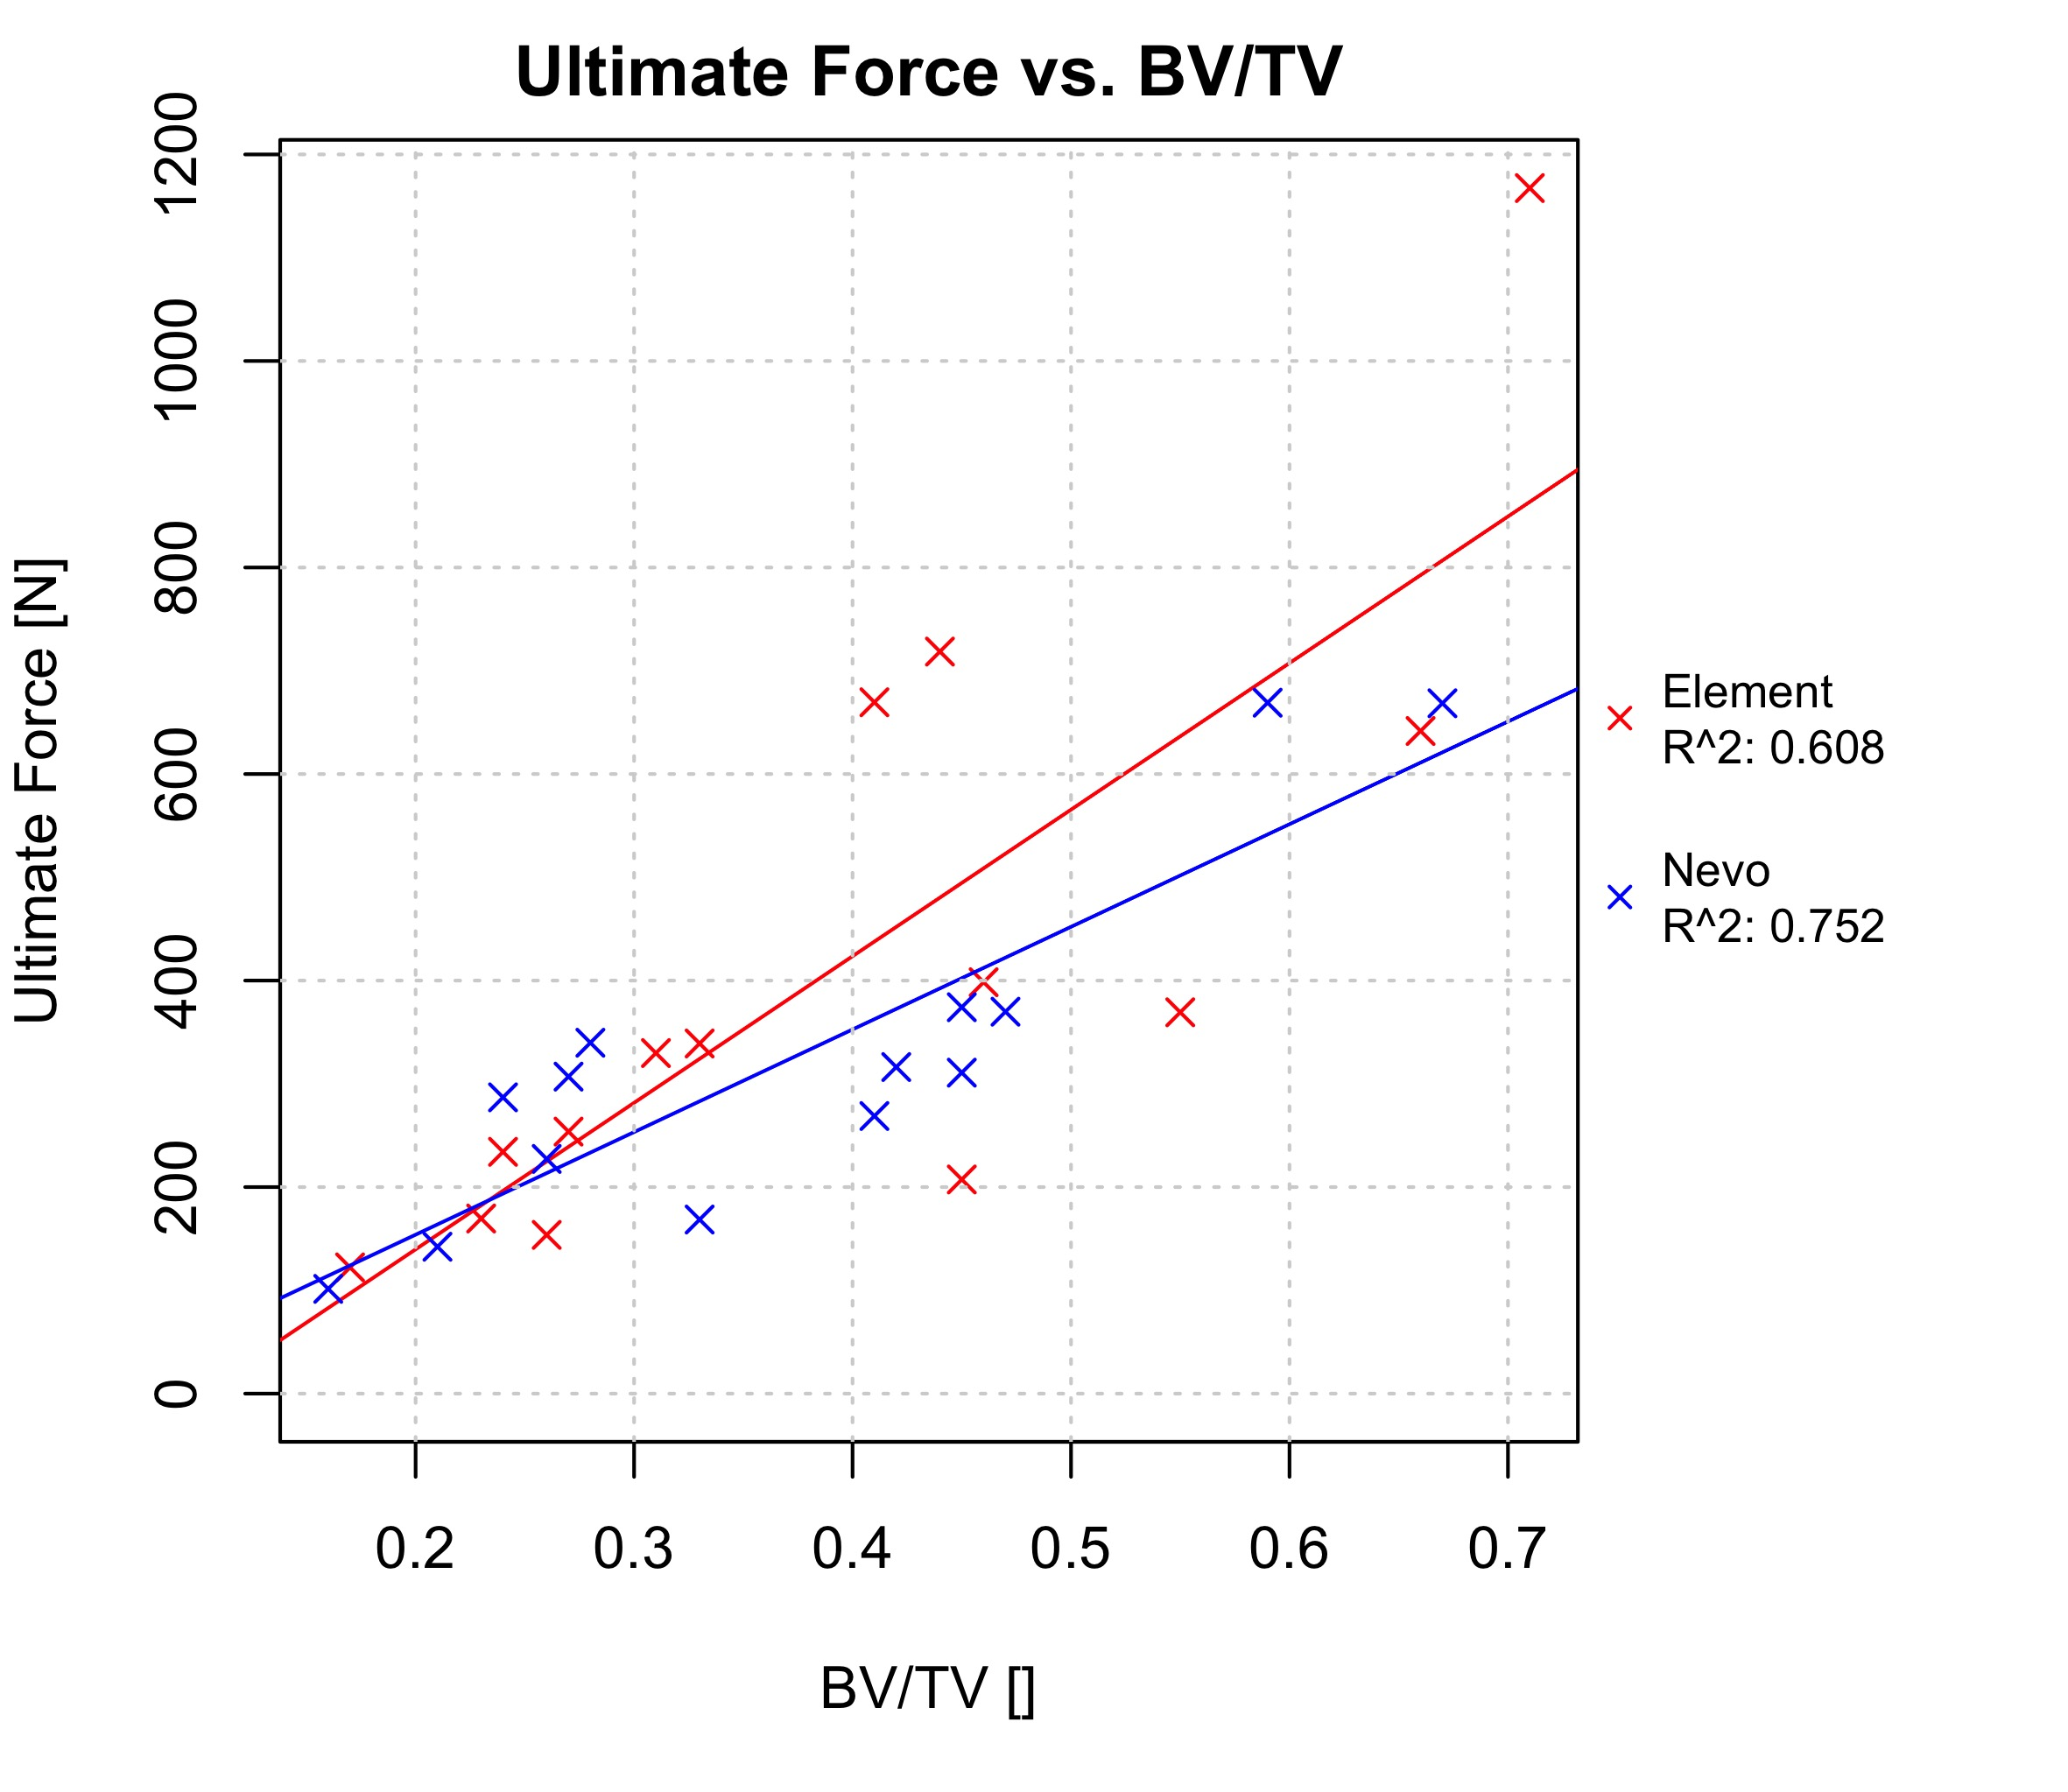
\includegraphics[width=0.49\textwidth]{figures/EXP_UF}}
\subfigure[]{\label{sublable2}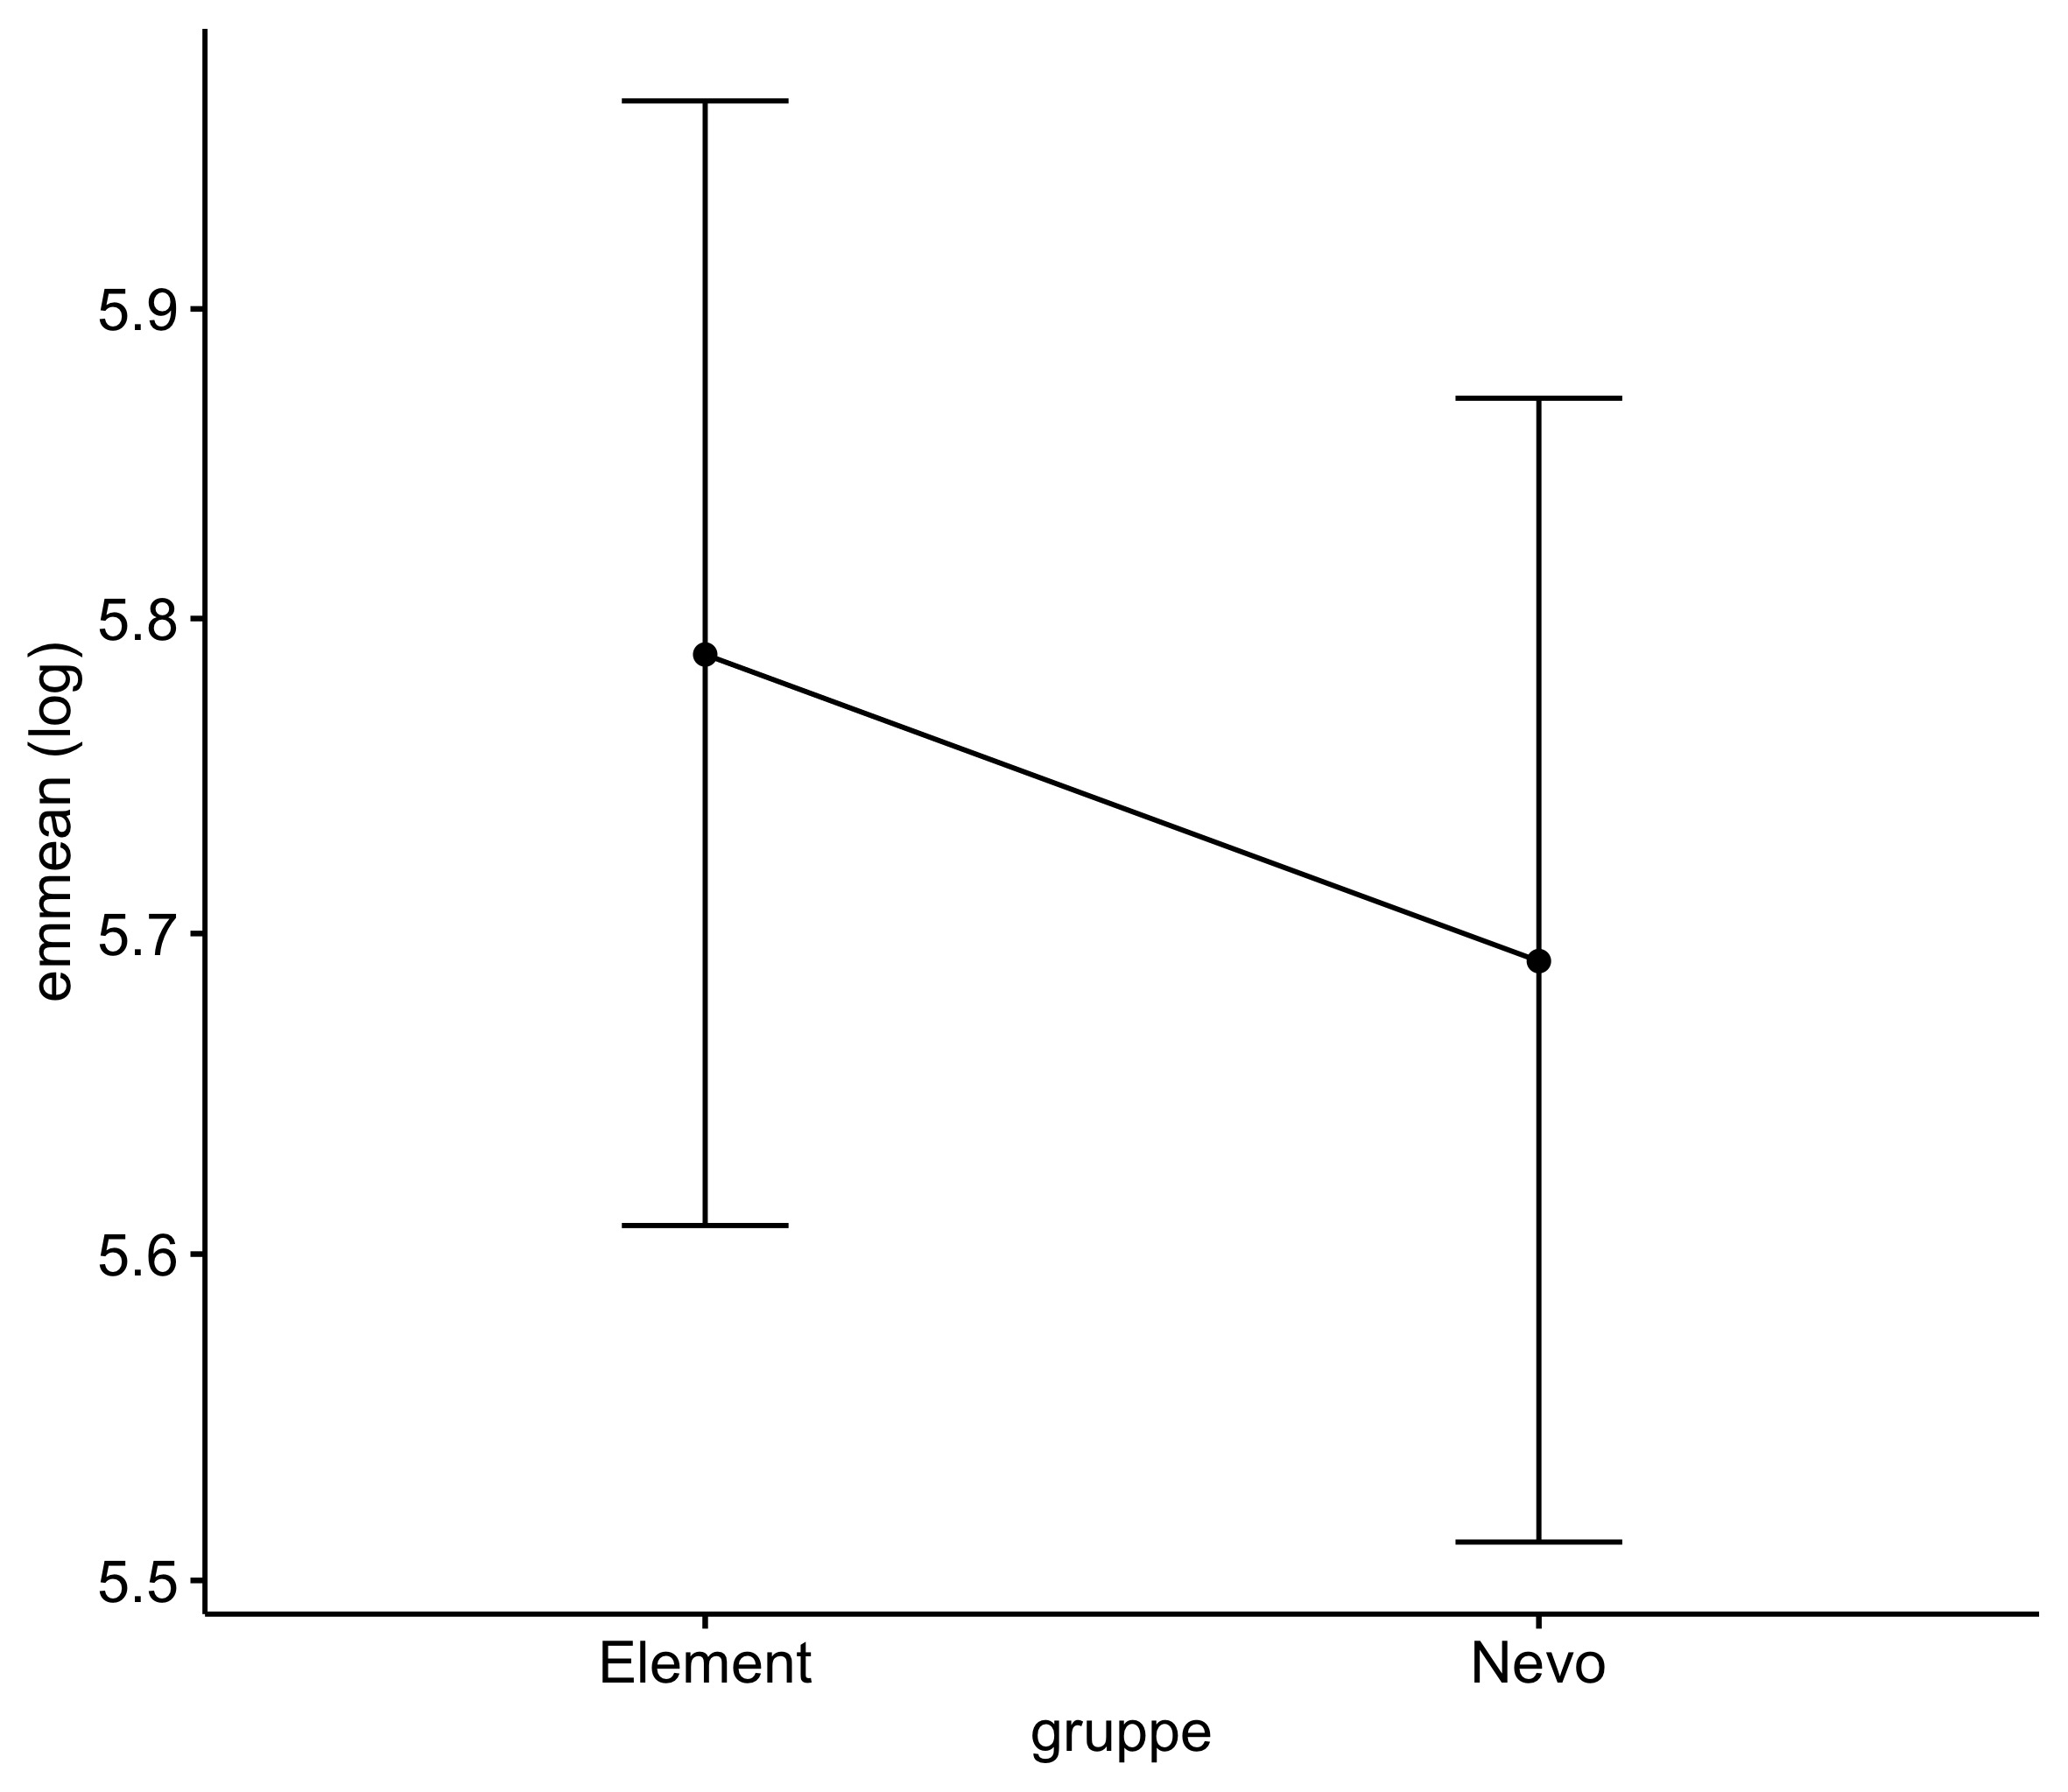
\includegraphics[width=0.49\textwidth]{figures/emmenas_UF}}
\captionof{figure}{(a): Ultimate force as a function of BV/TV with the individual linear regression model of each group. (b): Box plot of the estimated marginal means (emmeans or least square means) of each group after Bonferroni correction, controlled with BV/TV as the covariate.}
\label{fig:UF_exp}
\end{figure}
%
\begin{table}[H]
\centering
\resizebox{300pt}{!}{%
\begin{tabular}{|l|c|c|c|c||c|}
	\hline
	& \multicolumn{4}{c||}{individual lin. regression} & eval. ANCOVA (log)\\
	\hline 
	Group & $R^2$ & p-value & mean & CV & emmean $\pm$ 95\%conf.\\
	\hline
	ELEMENT & 0.67 & 2.20e-4 & 412.45 & 0.707 & 5.79 $\pm$ 0.18\\
	\hline
	NEVO & 0.71 & 9.41e-5 & 325.06 & 0.514 & 5.69 $\pm$ 0.18\\
	\hline
\end{tabular}
}
\caption{Results for the linear regression (RSE: residual standard error, CV: coefficient of variation) of the experimentally evaluated ultimate force values. And the evaluation of the ANCOVA by the emmeans after Bonferroni correction.}
\label{tab:uf_results}
\end{table}
%
\begin{table}[H]
\centering
\resizebox{200pt}{!}{%
\begin{tabular}{|l|c|c|c|c|c|c|}
	\hline 
	Effect & DFn & DFd & F & p & ges\\
	\hline
	\hline
	bvtv (log) & 1 & 25 & 60.915 & 3.68e-8 & 0.709\\
	\hline
	group & 1 & 25 & 0.619 & 4.39e-1 & 0.024\\
	\hline
\end{tabular}
}
\caption{Results from the ANCOVA analysis, controlling for BV/TV.}
\label{tab:uf_ancova}
\end{table}
%
%
% G1 and G3 showed a significant linear relationship between implantation ultimate force (UF) and BV/TV, where UF increases with increasing BV/TV. The linear relation in G2 is not significant but showed a strong tendency to the same behaviour as the others.\\
% \\
An overview of the statistical metrics can be found in the table~\ref{tab:uf_results}.
The ANCOVA indicated that the ultimate force was significantly related to the BV$/$TV of the sample, F(1,25)=60.915, p$<$0.001.
However, after controlling for the effect of BV$/$TV, there was no significant difference between the groups on ultimate force, F(1,25)$=$0.619, p$>$0.05.
See table~\ref{tab:uf_ancova} for details.

In a further analysis, the homogeneity of the regression slopes was analysed with an interaction term.
However, it was not statistically significant at p$>$0.05.

% The ANCOVA pointed out that globally (over all groups) the ultimate force was significantly related to the sample's BV$/$TV, F(1,24)$=$100.5, p$<$0.001. Further more, there was a significant difference between the groups on the ultimate force after controlling for the effect of the BV$/$TV, F(2,24)$=$34.8, p$<$0.001.\\
% Through the post hoc analysis it could be observed that the emmeans of the ultimate force is not significantly greater in G1 (701.0N) compared to G2 (608.0N), p$>$0.05. The mean ultimate force was significantly lower in G3 (283N) compared to G2 and G1. p$<$0.001.
%
%
%
\newpage
%
%
%
\chapter{Discussion, Limitations, and Conclusion}
%
%
%
\section{Discussion and Limitations}

% TODO: maybe add to the report why we think there are differences between expectations and results:
% notes new report:
% - Andere Belastungsart: vertikal nicht angewinkelt.
% - Rotationssteiffigkeit: dort nicht se ein grosser Unterschied.
% - Haben das Implantat nochmals geändert.

%
To summarise the results, only hypothesis one was not rejected, but hypotheses two and three had to be rejected.
An overview of the hypotheses in relation to the results can be seen in the table~\ref{tab:results_vs_h}.

During sample preparation we had an incident in the laboratory which resulted in samples not being frozen for 15 hours.
However, we estimate that this had no effect on the results as such thawing times are normal during sample preparation.

Three of the 28 implants could not be placed with the iChiro pro alone and had to be placed manually.
This prevented the measurement of the insertion torque and is the reason why the analysis with the insertion torque is only carried out on 25 samples.

Compared to the master thesis of~\cite{thierrin_primary_2022}, we used a different test sphere.
The thesis used a sphere that produced a lever arm that was 0.9mm smaller than the one specified in the ISO-14801 standard.
This is the reason why the design was changed compared to~\citet{thierrin_primary_2022}.

%
\begin{table}[H]
\centering
\begin{tabular}{|l|r|}
\hline
\multicolumn{2}{|l|}{The maximal … is higher for the SPI NEVO than the SPI ELEMENT} \\
\hline
H1: insertion torque & not rejected \\
\hline
\multicolumn{1}{|l|}{H2: stiffness} & rejected \\
\hline
H3: ultimate force & rejected \\
\hline
\end{tabular}
\caption{Overview of results in relation to the working hypotheses.}
\label{tab:results_vs_h}
\end{table}
%
%
\newpage
%
\section{Conclusion}
%
To summarise the results, only hypothesis one was not rejected, but hypotheses two and three had to be rejected.
This means that we were able to show that the stiffness and ultimate strength of the SPI NEVO is not statistically better than the SPI ELEMENT.

This is not what was initially expected according to the simulation results of~\cite{wili_virtual_2022}.
The reason for this difference between expectations and results can only be hypothesised at this stage.
A more detailed analysis would require finite element simulations with the newly obtained experimental data.

%The structural differences between the samples can lead to variances in the simulated results as it can be seen in the experiments. It seems that simulating only the min and max BV/TV samples is not sufficient for a proper evaluation by the FE-simulation.

%According to the ISQ measurements, for the group G3, there is no visible relationship with BV/TV and it is clearly different from Group G1 and Group G2. It leads to the conclusion that measuring ISQ values on not completely inserted implants is not very meaningful. 
\newpage
%
%
\appendix
\chapter{Appendix}
\newpage
\section*{Appendix A}

\newpage
%
%
%

%

%
%%%%%%%%%%%%%%%%%%%%%%%%%%%%%%%%%%%%%%%%%%%%%%%%%%%%%%%%%%%%%%%%%%%%%
\backmatter
\bibliographystyle{apalike}
\bibliography{biblio}

%%%%%%%%%%%%%%%%%%%%%%%%%%%%%%%%%%%%%%%%%%%%%%%%%%%%%%%%%%%%%%%%%%%%% 
%%%%%%%%%%%%%%%%%%%%%%%%%%%%%%%%%%%%%%%%%%%%%%%%%%%%%%%%%%%%%%%%%%%%% 
\end{document}
%%%%%%%%%%%%%%%%%%%%%%%%%%%%%%%%%%%%%%%%%%%%%%%%%%%%%%%%%%%%%%%%%%%%%
%%%%%%%%%%%%%%%%%%%%%%%%%%%%%%%%%%%%%%%%%%%%%%%%%%%%%%%%%%%%%%%%%%%%%
%%%%%%%%%%%%%%%%%%%%%%%%%%%%%%%%%%%%%%%%%%%%%%%%%%%%%%%%%%%%%%%%%%%%%
